\documentclass[12pt,oneside]{uhthesis}
\usepackage{subfigure}
\usepackage[ruled,lined,linesnumbered,titlenumbered,algochapter,spanish,onelanguage]{algorithm2e}
\usepackage{amsmath}
\usepackage{amssymb}
\usepackage{amsbsy}
\usepackage{caption,booktabs}
\usepackage[spanish]{babel}
\captionsetup{ justification = centering }
%\usepackage{mathpazo}
\usepackage{float}
\setlength{\marginparwidth}{2cm}
\usepackage{todonotes}
\usepackage{listings}
\usepackage{xcolor}
\usepackage{multicol}
\usepackage{graphicx}
\usepackage{hyperref}
\floatstyle{plaintop}
\restylefloat{table}
\addbibresource{Bibliography.bib}
% \setlength{\parskip}{\baselineskip}%
\renewcommand{\tablename}{Tabla}
\renewcommand{\listalgorithmcfname}{Índice de Algoritmos}
%\dontprintsemicolon
\SetAlgoNoEnd

\pagestyle{fancy}
\fancyhf{}
\fancyhf{}
\rhead{}
\lhead{Universidad de La Habana}
\rfoot{\thepage}

\definecolor{codegreen}{rgb}{0,0.6,0}
\definecolor{codegray}{rgb}{0.5,0.5,0.5}
\definecolor{codepurple}{rgb}{0.58,0,0.82}
\definecolor{backcolour}{rgb}{0.95,0.95,0.92}

\lstdefinestyle{mystyle}{
    backgroundcolor=\color{backcolour},   
    commentstyle=\color{codegreen},
    keywordstyle=\color{purple},
    numberstyle=\tiny\color{codegray},
    stringstyle=\color{codepurple},
    basicstyle=\ttfamily\footnotesize,
    breakatwhitespace=false,         
    breaklines=true,                 
    captionpos=b,                    
    keepspaces=true,                 
    numbers=left,                    
    numbersep=5pt,                  
    showspaces=false,                
    showstringspaces=false,
    showtabs=false,                  
    tabsize=4
}

\lstset{
    language=Python,
    basicstyle=\ttfamily,
    keywordstyle=\color{blue},
    commentstyle=\color{green},
    stringstyle=\color{red},
    showstringspaces=false,
    breaklines=true
}

\title{Análisis comparativo de métodos aproximados en solucionadores CDCL SAT}
\author{\\\vspace{0.25cm}Massiel Paz Otaño}
\advisor{\\\vspace{0.25cm}Dr. Luciano García Garrido} %\\\vspace{0.2cm}Nombre del segundo tutor}
\degree{Licenciada en Ciencia de la Computación}
\faculty{Facultad de Matemática y Computación}
\date{Fecha\\\vspace{0.25cm}\href{https://github.com/NinaSayers/Application-of-Computational-Logic-in-Problem-Solving.git}{github.com/NinaSayers/Application-of-Computational-Logic-in-Problem-Solving.git}}
\logo{Graphics/uhlogo}
\makenomenclature

\renewcommand{\vec}[1]{\boldsymbol{#1}}
\newcommand{\diff}[1]{\ensuremath{\mathrm{d}#1}}
\newcommand{\me}[1]{\mathrm{e}^{#1}}
\newcommand{\pf}{\mathfrak{p}}
\newcommand{\qf}{\mathfrak{q}}
%\newcommand{\kf}{\mathfrak{k}}
\newcommand{\kt}{\mathtt{k}}
\newcommand{\mf}{\mathfrak{m}}
\newcommand{\hf}{\mathfrak{h}}
\newcommand{\fac}{\mathrm{fac}}
\newcommand{\maxx}[1]{\max\left\{ #1 \right\} }
\newcommand{\minn}[1]{\min\left\{ #1 \right\} }
\newcommand{\lldpcf}{1.25}
\newcommand{\nnorm}[1]{\left\lvert #1 \right\rvert }
\renewcommand{\lstlistingname}{Ejemplo de código}
\renewcommand{\lstlistlistingname}{Ejemplos de código}

\begin{document}

\frontmatter
\maketitle

\begin{dedication}
\textit{Le dedico este trabajo de Diploma a mi mam\'a por su invaluable apoyo y a esa ni\~na que un d\'ia fui y que so\~naba con convertirse en cient\'ifica y resolver problemas dif\'iciles mediante grandes ideas.}
\end{dedication}
\begin{acknowledgements}
    Agradecimientos
\end{acknowledgements}
\begin{opinion}
    Opiniones de los tutores
\end{opinion}
\begin{resumen}
	Resumen en español
\end{resumen}

\begin{abstract}
	Resumen en inglés
\end{abstract}
\tableofcontents
\listoffigures
% \listoftables
% \listofalgorithms
\lstlistoflistings

\mainmatter

\chapter*{Introducción}\label{chapter:introduction}
\addcontentsline{toc}{chapter}{Introducción}
%Contexto histórico/social
El desarrollo de la lógica computacional como disciplina se enmarca en la revolución tecnológica del siglo XX, impulsada por la necesidad de resolver problemas complejos en ámbitos como la inteligencia artificial, la verificación de hardware y software, y la optimización industrial. La creciente demanda de sistemas automatizados capaces de procesar restricciones y tomar decisiones eficientes llevó a la comunidad científica a explorar métodos formales para modelar y resolver problemas combinatorios. En este escenario, la teoría de la complejidad computacional emergió como un pilar fundamental, especialmente tras la identificación de la clase NP-Completo por Cook en 1971, que transformó la comprensión de los límites de la computación.

%Antecedentes del problema científico
Los problemas con restricciones —aquellos que requieren satisfacer un conjunto de condiciones lógicas— han sido centrales en áreas como la planificación, la criptografía y el diseño de circuitos. El problema de satisfacibilidad booleana (SAT), demostrado por Cook como el primer problema NP-Completo, se convirtió en la piedra angular para estudiar la viabilidad de soluciones eficientes. Aunque los primeros algoritmos para SAT, como el método de Davis-Putnam (DP) y su evolución, Davis-Putnam-Logemann-Loveland (DPLL), sentaron las bases de los \textit{solvers}, su eficiencia se veía limitada por la explosión combinatoria en instancias complejas. La presencia de cláusulas unitarias, la selección subóptima de variables y el retroceso (backtrack) cronológico exponían claras debilidades, especialmente en problemas con miles de variables.

%Breve presentación de la problemática
A pesar de los avances, los SAT \textit{solvers} clásicos enfrentaban un desafío crítico: escalar sin sacrificar completitud. Esto motivó la búsqueda de mejoras heurísticas y estratégicas, como el aprendizaje de cláusulas y el \textit{backtrack} no cronológico, que culminaron en el surgimiento del paradigma Conflict-Driven Clause Learning (CDCL). CDCL no solo optimizó la exploración del espacio de soluciones, sino que introdujo mecanismos para evitar repeticiones de conflictos, marcando un hito en la resolución práctica de problemas NP-Completos. 

%Sin embargo, la eficacia de estos algoritmos depende en gran medida de estrategias de selección de variables, como VSIDS (Variable State Independent Decaying Sum) y DLIS (Dynamic Largest Individual Sum), cuyas ventajas comparativas siguen siendo objeto de debate.

El núcleo de la eficiencia de los SAT \textit{solvers} modernos reside, sin lugar a dudas, en su capacidad para reducir el espacio de búsqueda de forma inteligente. Sin embargo, incluso con técnicas como CDCL, un desafío persiste: la selección óptima de variables. Esta elección determina la dirección en la que el algoritmo explora el árbol de decisiones, y una estrategia subóptima puede llevar a ciclos de conflicto-reparación redundantes, incrementando exponencialmente el tiempo de ejecución. En problemas NP-Completos, donde el número de posibles asignaciones crece como $2^n$ (con $n$ variables), una heurística de selección inadecuada convierte instancias resolubles en minutos en problemas intratables.

%¿Por qué la selección de variables es crítica?
En CDCL, tras cada conflicto, el solucionador aprende una cláusula nueva para evitar repeticiones. No obstante, la eficacia de este aprendizaje depende de qué variables se eligieron para bifurcar el espacio de soluciones. Si se seleccionan variables irrelevantes o poco conectadas a los conflictos, las cláusulas aprendidas serán débiles o redundantes, limitando su utilidad. Así, la selección de variables no es solo una cuestión de orden, sino de calidad de la exploración.

Dos de las heurísticas de selección de variables son VSIDS (Variable State Independent Decaying Sum) y DLIS (Dynamic Largest Individual Sum). Ambas, son aproximaciones \textit{greedy}, dado que optimizan localmente (paso a paso) sin garantizar una solución global óptima. Su eficacia depende de cómo la estructura del problema se alinee con sus criterios. Por una parte, VSIDS asigna un puntaje a cada variable, incrementándolo cada vez que aparece en una cláusula involucrada en un conflicto. Periódicamente, estos puntajes se reducen (\textit{decaimiento} exponencial), priorizando variables activas recientemente. Por otra parte, DLIS calcula, para cada literal (variable o su negación), el número de cláusulas no satisfechas donde aparece. Selecciona el literal con mayor frecuencia y asigna su variable correspondiente.

En los CDCL SAT \textit{solvers} se ha observado que el tiempo de ejecución puede seguir una distribución de ``cola pesada'' (\textit{heavy-tailed distribution}), lo que significa que el solucionador puede quedarse atascado en un camino de búsqueda improductivo por un tiempo prolongado. En aras de resolver este problema, surge la estrategia \textit{restart}, la cual borra parte del estado del \textit{solver} a intervalos determinados durante su ejecución. Su principal objetivo es reorientar la búsqueda y aprovechar el conocimiento acumulado mientras se evita profundizar en regiones improductivas del árbol de búsqueda. Al reiniciar, el resolvedor puede escapar de una dirección de búsqueda desventajosa y tener una ``segunda oportunidad'' para encontrar una solución más rápidamente.



%VSIDS

%Fortaleza: Adaptabilidad dinámica. Al enfocarse en variables vinculadas a conflictos recientes, explota patrones locales en problemas estructurados (ej: verificaciones de circuitos).

%Debilidad: Puede ignorar variables críticas en regiones no exploradas del espacio.

%DLIS (Dynamic Largest Individual Sum):

%Mecanismo: Calcula, para cada literal (variable o su negación), el número de cláusulas no satisfechas donde aparece. Selecciona el literal con mayor frecuencia y asigna su variable correspondiente.

%Fortaleza: Basado en la estructura estática del problema, ideal para instancias con distribución uniforme de restricciones (ej: SAT aleatorio).

%Debilidad: No adapta su estrategia durante la ejecución, volviéndose ineficaz en problemas con dependencias ocultas o jerarquías.

%Actualidad
Hoy, aunque los SAT solucionadores basados en CDCL dominan aplicaciones críticas, desde la verificación formal de chips hasta la síntesis de programas, su rendimiento varía significativamente según el tipo de problema (p. ej., aleatorios vs. estructurados) y las heurísticas empleadas. Mientras VSIDS prioriza variables recientemente involucradas en conflictos —útil en problemas con alta estructura local—, DLIS enfatiza la frecuencia de aparición de literales, mostrando ventajas en dominios con distribución uniforme de restricciones. Esta dualidad plantea preguntas clave: ¿bajo qué métricas (tiempo de ejecución, memoria, escalabilidad) una estrategia supera a la otra? ¿Cómo influye la naturaleza del problema en su eficiencia?

%Novedad científica
Esta tesis aporta una comparación sistemática entre VSIDS y DLIS, alternando entre el uso de \textit{restar} dentro del entorno CDCL que ofrece el solucionador CaDiCaL, evaluando su desempeño en problemas heterogéneos (industriales, aleatorios y académicos). A diferencia de estudios previos, se integran métricas adaptativas que consideran no solo el tiempo de resolución, sino también el impacto de las caracter\'isticas de los problemas. Además, se propone un marco teórico amplio para comprender la evoluci\'on algor\'itmica de los CDCL SAT \textit{solvers}, entender algunas de las heur\'isticas que se emplean en los solucionadores modernos, espec\'ificamente en CaDiCaL, y clasificar problemas según su afinidad heurística, contribuyendo a la selección informada de algoritmos en aplicaciones reales.

%Importancia teórica y práctica
Teóricamente, este trabajo profundiza en la relación entre estructura de problemas y heurísticas, enriqueciendo la comprensión de CDCL. Prácticamente, ofrece directrices para ingenieros y desarrolladores de \textit{solvers}, optimizando recursos en áreas como la verificación de \textit{software} o la logística, donde minutos de mejora equivalen a ahorros millonarios.

%Diseño teórico
Como problema científico se plantea la ineficiencia de los SAT solucionadores ante problemas con distintas estructuras, asociada a la selección subóptima de variables, influenciada o no por t\'ecnicas de reinicio. El objeto de estudio se centrar\'a en algoritmos CDCL con estrategis VSIDS, DLIS y \textit{restart}. Esta tesis tiene como objetivos:
\begin{itemize}
    \item Analizar el impacto de VSIDS y DLIS, con y sin reinicio, en el rendimiento de CDCL.
    \item Establecer correlaciones entre tipos de problemas y heurísticas.
    \item Establecer correlaiones entre tipos de problemas y resultados de las heur\'isticas.
\end{itemize}
El campo de acci\'on de esta tesis versa sobre la Lógica computacional aplicada a la resolución de problemas con restricciones.
Como hipótesis se plantea que: El rendimiento de VSIDS y DLIS con y sin \textit{restart} varía significativamente según la densidad de restricciones, el tama\~no promedio de cl\'ausula y la cantidad de variables.
Esta investigación busca no solo esclarecer el debate entre VSIDS y DLIS, sino también sentar bases para el diseño de heurísticas adaptativas, impulsando la próxima generación de resolvedores.

%Estructuración del trabajo
El documento se organiza en cinco capítulos:
\begin{itemize}
    \item \textbf{Cap\'itulo 1} Revisión teórica de los principales algoritmos usados en los SAT solvers, algunas heur\'isticas empleadas en los \textit{solvers} modernos haciendo \'enfasis en CaDiCaL, y de las categor\'ias de problemas usadas en el an\'alisis de eficiencia de los solucionadores SAT.
    \item \textbf{Cap\'itulo 2} Detalles de implementaci\'on de las heur\'isticas en CaDiCaL, del generador de problemas y de los an\'alisis estad\'isticos empleados.
    \item \textbf{Cap\'itulo 3} Resultados de los experimentos.
    \item \textbf{Cap\'itulo 4} Conclusiones y recomendaciones.
\end{itemize}


\chapter{Marco Teórico}\label{chapter:state-of-the-art}

\section{Fundamentos de los Problemas de Satisfacción de Restricciones y SAT}
\label{sec:fundamentos-sat-csp}

Los Problemas de Satisfacción de Restricciones (CSPs) constituyen un paradigma fundamental para modelar desafíos combinatorios en inteligencia artificial, investigación operativa y ciencias de la computación. Formalmente, un CSP se define mediante una tripleta $(V,D,C)$, donde $V$ es un conjunto de variables, $D$ sus dominios discretos finitos, y $C$ un conjunto de restricciones que limitan las combinaciones válidas de valores \textbf{39}. Por ejemplo, en un problema de asignación de horarios, $V$ representaría cursos, $D$ los horarios disponibles, y $C$ las reglas que evitan superposiciones. La solución óptima no solo satisface todas las restricciones, sino que también optimiza criterios como la utilización de recursos \textbf{40}.

\subsection{SAT como Caso Especial de CSP y su NP-Completitud}
El Problema de la Satisfacibilidad Booleana (SAT) emerge como un CSP restringido donde los dominios son binarios (${0,1}$) y las restricciones se expresan en Forma Normal Conjuntiva (FNC) \textbf{43}. Una fórmula en FNC es una conjunción de cláusulas, donde cada cláusula es una disyunción de literales (variables o sus negaciones) \textbf{6}. Determinar si existe una asignación de valores que satisfaga todas las cláusulas equivale a resolver un CSP binario con restricciones específicas.

La relevancia teórica de SAT radica en su condición de problema NP-completo, demostrada por Cook y Levin en 1971 \textbf{2,24}. Este estatus implica dos consecuencias cruciales: primero, cualquier problema en NP puede reducirse a SAT en tiempo polinomial \textbf{26}; segundo, la existencia de un algoritmo polinomial para SAT implicaría $P=NP$, colapsando la jerarquía de complejidad \textbf{2}. Aunque en la práctica los solvers modernos resuelven instancias con millones de variables \textbf{3}, en el peor caso SAT conserva una complejidad exponencial inherente \textbf{27}.

\subsection{Ineficiencias Fundamentales de SAT}
\label{subsec:ineficiencia-sat}

El método de fuerza bruta para SAT —evaluar todas $2^n$ asignaciones posibles mediante tablas de verdad— ilustra su naturaleza intratable en el peor caso \textbf{19}. Esta explosión combinatoria se agrava en fórmulas sin estructura discernible, donde técnicas como la propagación unitaria o el aprendizaje de cláusulas tienen impacto limitado \textbf{30}. Por ejemplo, en instancias aleatorias de 3-SAT cerca del umbral de fase (aproximadamente 4.26 cláusulas por variable \textbf{30}), los algoritmos clásicos como DPLL exhiben un crecimiento exponencial en el tiempo de ejecución \textbf{27}.

Aun así, SAT destaca como herramienta práctica gracias a dos factores: (1) la capacidad de codificar CSPs genéricos en FNC mediante técnicas como \textit{encodings} directos o Tseitin \textbf{44}, y (2) el desarrollo de solvers CDCL que explotan regularidades empíricas en instancias industriales \textbf{3}. Esta dualidad entre dificultad teórica y éxito práctico sitúa a SAT en el núcleo de aplicaciones como verificación de hardware, planificación autónoma y criptoanálisis \textbf{39}.

\subsection{Relación Práctica entre CSPs y SAT}
\label{subsec:csp-sat-relacion}

Aunque los CSPs permiten modelar problemas con dominios arbitrarios y restricciones globales —ventaja frente a la rigidez booleana de SAT—, su resolución nativa mediante métodos como \textit{backtracking} o consistencia de arco sufre de limitaciones similares en escalabilidad \textbf{46}. Por ello, una estrategia común consiste en traducir CSPs a SAT, aprovechando décadas de optimizaciones en solvers CDCL \textbf{44}. Estudios empíricos demuestran que codificaciones eficientes (e.g., \textit{order encoding} para restricciones de orden) reducen hasta un 60\% el tiempo de resolución frente a enfoques CSP nativos \textbf{45}.

No obstante, esta traducción no está exenta de trade-offs. Mientras SAT favorece restricciones locales y cláusulas pequeñas, los CSPs manejan eficientemente restricciones globales (e.g., \textit{alldifferent}) mediante propagadores especializados \textbf{46}. Por ejemplo, en problemas de asignación de turnos hospitalarios, un modelo CSP con restricciones de recurso puede resolver instancias en minutos, mientras su traducción a SAT requiere horas debido a la explosión de cláusulas \textbf{46}. Esta dicotomía subraya la importancia de seleccionar el paradigma adecuado según la estructura del problema.

\subsection{Enfoques de Solución: CP, MILP y SAT}
\label{subsec:enfoques-solucion}

La resolución de CSPs y SAT se enmarca en tres metodologías principales:
\begin{itemize}
\item \textbf{Programación con Restricciones (CP)} \textbf{40}: Combina búsqueda sistemática con propagación de restricciones, ideal para dominios discretos y restricciones no lineales.
\item \textbf{Programación Entera Mixta (MILP)} \textbf{40}: Utiliza relajaciones lineales y técnicas branch-and-bound, óptima para problemas con estructura matemática explícita.
\item \textbf{Satisfacibilidad Booleana (SAT)} \textbf{44}: Emplea algoritmos CDCL con aprendizaje de cláusulas, eficaz para problemas binarios o altamente restringidos.
\end{itemize}

Cada enfoque tiene un nicho de aplicabilidad. Por ejemplo, CP domina en scheduling con restricciones complejas, MILP en optimización logística lineal, y SAT en verificación formal donde la traducibilidad a FNC es natural \textbf{39,40}. La elección depende críticamente de la capacidad para explotar la estructura subyacente del problema —factor que explica el éxito paradójico de SAT pese a su complejidad teórica \textbf{3}.

%\begin{figure}[h]
%\centering
%\includegraphics[width=0.85\textwidth]{sat-csp-comparison.pdf}
%\caption{Comparación de tiempos de resolución entre modelos CSP nativos y codificaciones SAT para instancias del problema N-Reinas (Fuente: Elaboración propia basada en benchmarks de \textbf{45}).}
%\label{fig:sat-csp-comp}
%\end{figure}

Esta sección sienta las bases para analizar en detalle la evolución de los SAT solvers (Sección \ref{sec:evolucion-sat-solvers}), donde se explorará cómo técnicas como CDCL superaron las ineficiencias teóricas mediante innovaciones algorítmicas pragmáticas.

\section{Evolución de los SAT \textit{solvers}: Principio de Resolución, DP, DPLL y CDCL}
\label{sec:evolucion-sat-solvers}

La historia de los SAT \textit{solvers} representa un hito en la ciencia computacional, transformando un problema teóricamente intratable en una herramienta práctica de amplio uso industrial. Esta evolución se sustenta en tres pilares algorítmicos: el Principio de Resolución, los métodos Davis-Putnam (DP) y Davis-Putnam-Logemann-Loveland (DPLL), y la revolución moderna impulsada por los solucionadores de aprendizaje de cláusulas dirigido por conflictos (CDCL). Este recorrido no solo refleja avances técnicos, sino una comprensión profunda de cómo combinar teoría y pragmatismo para superar las barreras de complejidad inherentes al problema de la satisfacibilidad booleana (SAT)\footnote{Problema NP-completo que busca determinar si existe una asignación de verdad que satisfaga una fórmula lógica dada.}.

\subsection{Principio de Resolución: Fundamento Teórico}
El Principio de Resolución (PR), propuesto inicialmente en el contexto de la lógica proposicional, constituye la base teórica de muchos algoritmos SAT. Este principio permite derivar nuevas cláusulas a partir de un par de cláusulas existentes que contengan literales complementarios, reduciendo progresivamente la fórmula hasta detectar una contradicción o verificar su satisfacibilidad. Aunque teóricamente completo para fórmulas en Forma Normal Conjuntiva (FNC), su aplicación directa resulta impráctica debido al crecimiento explosivo en el número de cláusulas generadas \textbf{12}. No obstante, su valor conceptual sentó las bases para métodos más refinados.

\subsection{Algoritmo Davis-Putnam (DP): Primer Intento Práctico}
Introducido en 1960 \textbf{5}, el algoritmo DP fue el primer esfuerzo sistemático para operacionalizar el PR en un marco computacional. Su estrategia se centraba en la eliminación iterativa de variables mediante dos reglas: (1) \textit{eliminación de literales puros} (asignar valores a variables que aparecen con un único signo en todas las cláusulas) y (2) \textit{resolución dirigida} para eliminar variables seleccionadas. Aunque evitaba el espacio exponencial de las tablas de verdad, su dependencia de la resolución lo hacía vulnerable a explosiones combinatorias en el número de cláusulas intermedias \textbf{12}. Este defecto limitó su aplicabilidad a instancias pequeñas, pero demostró que la combinación de inferencia lógica y manipulación algebraica podía abordar SAT de manera estructurada.

\subsection{Algoritmo DPLL: Búsqueda Inteligente con Retroceso}
En 1962, Davis, Putnam, Logemann y Loveland refinaron DP mediante un giro paradigmático: reemplazaron la resolución explícita por una \textit{búsqueda con retroceso} en el espacio de asignaciones, dando origen al algoritmo DPLL \textbf{12}. Este método integra tres componentes clave:
\begin{itemize}
\item \textbf{Propagación Unitaria}: Asignación forzada de literales en cláusulas unitarias, reduciendo la fórmula antes de tomar decisiones.
\item \textbf{Eliminación de Literales Puros}: Optimización heredada de DP para simplificar la fórmula.
\item \textbf{Bifurcación con Retroceso}: Elección heurística de valores para variables no determinadas, seguida de retroceso ante conflictos.
\end{itemize}

Al operar como un recorrido en profundidad del árbol de decisiones, DPLL evita el costo de memoria de DP y se convirtió en el núcleo de los SAT \textit{solvers} clásicos \textbf{7}. Sin embargo, su eficiencia se veía mermada en problemas industriales debido a la exploración redundante de subespacios conflictivos y la ausencia de mecanismos para capitalizar información de conflictos pasados \textbf{8}. Estas limitaciones motivaron la búsqueda de estrategias que trascendieran el paradigma de fuerza bruta.

\subsection{CDCL: La Revolución de los \textit{Solvers} Modernos}
\label{subsec:cdcl}

El algoritmo CDCL emergió como solución a las limitaciones estructurales de DPLL en instancias industriales. Dos innovaciones fueron fundamentales: el \textit{aprendizaje de cláusulas} y el \textit{retroceso no cronológico} \textbf{12}. El primero transforma los conflictos en conocimiento estructural mediante el análisis de implicaciones, generando cláusulas que encapsulan inconsistencias para podar futuras ramas de búsqueda \textbf{17}. El segundo permite saltar a niveles de decisión estratégicos, evitando la exploración redundante de subárboles irrelevantes \textbf{6}. Juntos, estos mecanismos resolvieron tres problemas críticos de DPLL: la explosión combinatoria por conflictos repetidos, la falta de adaptación heurística durante la búsqueda y la ineficiencia del retroceso cronológico \textbf{5,7,8}.

\subsubsection{Mejoras Clave en CDCL: Heurísticas y Estrategias}
\label{subsubsec:mejoras-cdcl}

Si bien CDCL superó teóricamente a DPLL, su eficacia práctica requirió mejoras adicionales. Entre ellas destacan las heurísticas de selección de variables, estrategias de reinicio adaptativo y optimizaciones en la propagación unitaria.

Las \textit{heurísticas de selección de variables} representan un equilibrio entre complejidad teórica y pragmatismo. DLIS (\textit{Dynamic Largest Individual Sum}), uno de los primeros enfoques dinámicos \textbf{17}, prioriza variables frecuentes en cláusulas insatisfechas mediante conteos estáticos \textbf{18}. Aunque intuitivo, su costo computacional lineal ($O(n)$) y su incapacidad para adaptarse a la dinámica de búsqueda lo limitaron en instancias industriales \textbf{22}. VSIDS (\textit{Variable State Independent Decaying Sum}), en contraste, introdujo un modelo basado en actividades dinámicas con decaimiento exponencial \textbf{27}. Al incrementar puntuaciones de variables en conflictos recientes y aplicar factores de olvido periódicos \textbf{28}, VSIDS logró un balance empírico entre adaptación y costo computacional ($O(1)$ mediante colas de prioridad) \textbf{30}. Sin embargo, ambas heurísticas son aproximaciones: DLIS por su simplicidad estática, VSIDS por depender de correlaciones no garantizadas entre conflictos y tiempo de resolución \textbf{10,35}.

Las \textit{estrategias de reinicio adaptativo} surgieron para contrarrestar el estancamiento en regiones locales del espacio de búsqueda, un efecto colateral de heurísticas como VSIDS \textbf{44}. Técnicas como los reinicios LBD-driven en Glucose \textbf{14} vinculan la frecuencia de reinicios al Literal Block Distance promedio de cláusulas aprendidas, indicador indirecto de estancamiento. Métodos más sofisticados, como MAB (\textit{Multi-Armed Bandit}) en Kissat \textbf{37}, emplean aprendizaje en línea para seleccionar políticas de reinicio óptimas según el contexto de búsqueda. Estas estrategias reducen hasta un 70\% el tiempo de resolución en instancias modulares al reorientar la exploración sin perder cláusulas aprendidas críticas \textbf{21}.

En la \textit{propagación unitaria}, optimizaciones como el esquema de Dos Literales Vigilados (TWL) \textbf{29} minimizaron el costo de detectar cláusulas unitarias, evitando inspeccionar el 90\% de las cláusulas en cada asignación \textbf{12}. Técnicas posteriores como CFUP (\textit{Core First Unit Propagation}) \textbf{96} priorizaron cláusulas con LBD $\leq$ 7, basándose en la observación empírica de que el 80\% de los conflictos ocurren en estas estructuras. Si bien CFUP carece de fundamentación teórica, su efectividad práctica lo consolidó como estándar en solvers como CaDiCaL \textbf{30}.

\subsubsection{Otras Contribuciones Relevantes}
\label{subsubsec:otras-mejoras}

El ecosistema de mejoras en CDCL incluye avances complementarios. La gestión de cláusulas aprendidas mediante métricas como LBD permitió eliminar cláusulas redundantes y reciclar aquellas con alto valor predictivo (\textit{glue clauses}) \textbf{14-17}. La integración con búsqueda local, mediante técnicas como \textit{re-phasing} basado en frecuencias de conflicto \textbf{1}, mejoró hasta un 40\% el rendimiento en instancias satisfacibles. En paralelo, meta-heurísticas como AutoSAT \textbf{35} exploraron el uso de modelos de lenguaje grande (LLMs) para optimizar parámetros dinámicos, aunque su adopción práctica sigue siendo incipiente.

%\begin{figure}[h]
%\centering
%\includegraphics[width=0.8\textwidth]{cdcl-evolucion.pdf}
%\caption{Reducción acumulada en tiempo de ejecución atribuible a mejoras en CDCL (Fuente: Análisis de resultados de SAT Competition 2010-2023).}
%\label{fig:cdcl-evol}
%\end{figure}

\subsection{CDCL como Motor para Problemas con Restricciones}
La efectividad de CDCL en CSPs depende críticamente de su arquitectura adaptativa. VSIDS explota patrones emergentes en restricciones codificadas, mientras los reinicios LBD-driven manejan la modularidad típica de estos problemas \textbf{15,21}. Técnicas como CFUP, al priorizar cláusulas "core", reflejan jerarquías implícitas en redes de restricciones \textbf{96}. Esta sinergia explica por qué solvers como Kissat y Glucose se han convertido en motores subyacentes para sistemas de verificación y planificación industrial \textbf{12}.

%\subsection{CDCL como Motor para Problemas con Restricciones}
%La versatilidad de CDCL trasciende SAT: al codificar Problemas de Satisfacción de Restricciones (CSPs) en FNC, estos \textit{solvers} actúan como oráculos para la clase NP \textbf{8}. Su capacidad para generar \textit{testigos} (soluciones) o \textit{núcleos insatisfacibles} (subconjuntos conflictivos) los hace herramientas clave en verificación formal, planificación y optimización combinatoria. Además, técnicas como el aprendizaje de cláusulas han influido en el diseño de solucionadores híbridos que integran SAT con dominios específicos \textbf{12} La elección de heurísticas como VSIDS y políticas de reinicio adaptativo resulta crucial al codificar CSPs en SAT, donde la estructura de restricciones se traduce en patrones específicos de aparición de variables que estas técnicas explotan \textbf{15,22}..

\subsection{Conclusión: De la Teoría a la Revolución Práctica}
La transición desde el PR y DP hasta CDCL ilustra cómo innovaciones algorítmicas pueden superar barreras teóricas aparentemente infranqueables. Mientras DPLL sentó las bases de la integración búsqueda-inferencia, CDCL introdujo un paradigma de \textit{aprendizaje reflexivo}, donde cada conflicto alimenta la inteligencia del solver. Esta evolución, respaldada por mejoras en heurísticas y estructuras de datos, ha convertido a los SAT \textit{solvers} en pilares de la computación moderna, demostrando que incluso problemas NP-completos pueden abordarse eficientemente en escenarios prácticos \textbf{5,7,11}.


\section{Parámetros de Evaluación para Solvers CDCL: Taxonomía de \textit{Benchmarks}}
\label{sec:tipos-problemas}

La evaluación rigurosa de solvers CDCL —particularmente en el análisis comparativo de heurísticas como VSIDS y DLIS, estrategias de reinicio y selección de cláusulas unitarias— requiere una taxonomía precisa de instancias SAT. Estas se clasifican no solo por su origen, sino por propiedades intrínsecas que revelan fortalezas y limitaciones algorítmicas \textbf{15,17}.

\subsection{Clasificación por Origen y Estructura}
Las competiciones anuales de SAT (\textit{SAT Competition}) establecen cuatro categorías canónicas \textbf{17}:

\textbf{Instancias de Aplicación}: Derivadas de problemas industriales como verificación de circuitos o planificación logística \textbf{11}, exhiben estructuras modulares y \textit{backdoors} pequeños —subconjuntos de variables cuya asignación correcta simplifica drásticamente la solución \textbf{21,23}. Estas características permiten a heurísticas dinámicas como VSIDS explotar patrones locales mediante el rastreo de conflictos recientes \textbf{20}.

\textbf{Instancias Combinatorias Dificultosas}: Construidas artificialmente para desafiar a los solvers (e.g., codificaciones del principio del palomar) \textbf{16}, carecen de la estructura implícita de las aplicaciones reales pero poseen simetrías y dependencias globales que prueban la capacidad de generalización de las heurísticas \textbf{19}.

\textbf{Instancias Aleatorias}: Generadas mediante modelos como Random k-SAT \textbf{17}, su falta de estructura las convierte en un desafío para CDCL, donde técnicas como el aprendizaje de cláusulas muestran eficacia limitada \textbf{21}. Estas instancias son críticas para evaluar el desempeño en ausencia de sesgos estructurales.

\textbf{Instancias Ágiles}: Resultantes de la conversión de problemas de lógicas superiores a SAT (\textit{bit-blasting}) \textbf{19}, testean la capacidad de manejar fórmulas con alta densidad de cláusulas y variables auxiliares.

\subsection{Clasificación por Satisfacibilidad y Propiedades Estructurales}
La naturaleza SAT o UNSAT de una instancia influye significativamente en el comportamiento del solver. Mientras las instancias SAT benefician a heurísticas que priorizan la exploración de asignaciones prometedoras (e.g., VSIDS con \textit{phase saving}), las UNSAT requieren estrategias que aceleren la refutación mediante cláusulas aprendidas de alto impacto \textbf{41}.

Propiedades estructurales como la modularidad, \textit{treewidth} y presencia de \textit{backbones} (variables con valor fijo en todas las soluciones) \textbf{20,22} ofrecen insights adicionales. Por ejemplo, instancias con alta modularidad —típicas en aplicaciones industriales— permiten a los reinicios adaptativos reorientar la búsqueda hacia comunidades no exploradas \textbf{21}, mientras que un \textit{treewidth} bajo correlaciona con tiempos de resolución reducidos debido a la eficiencia de la propagación unitaria \textbf{20}.

\subsection{Densidad y Transición de Fase}
La relación cláusulas/variables (densidad) determina la dificultad en instancias aleatorias. Para 3-SAT, la transición de fase alrededor de 4.27 cláusulas por variable \textbf{25} marca el pico de complejidad, donde métodos como DLIS —basados en frecuencias estáticas— fallan ante la ausencia de patrones explotables \textbf{17}. En contraste, VSIDS combinado con reinicios dinámicos (\textit{LBD-driven}) logra navegar estas regiones mediante un balance entre explotación local y exploración global \textbf{21}.

En instancias estructuradas, sin embargo, densidades altas no siempre implican mayor dificultad. Codificaciones compactas de problemas como el coloreado de grafos pueden ser resueltas eficientemente si los \textit{solvers} identifican \textit{backdoors} mediante heurísticas sensibles al contexto \textbf{23}.

\subsection{Relevancia para la Evaluación de Heurísticas}
La elección de \textit{benchmarks} es crucial al comparar técnicas como VSIDS y DLIS. Mientras DLIS —dependiente de conteos estáticos de aparición— rinde mejor en instancias aleatorias lejos de la transición de fase \textbf{18}, VSIDS domina en aplicaciones reales gracias a su adaptación dinámica \textbf{30}. Estrategias de reinicio como MAB \textbf{37} muestran ventajas en instancias modulares, donde reiniciar preservando cláusulas \textit{glue} acelera la cobertura del espacio de búsqueda \textbf{21}.

Propiedades como la presencia de \textit{backbones} o bajo \textit{treewidth} permiten diseccionar el impacto de técnicas específicas. Por ejemplo, la selección de cláusulas unitarias mediante CFUP \textbf{96} reduce hasta un 40\% el tiempo en instancias con alta densidad de cláusulas \textit{core} ($LBD \leq 7$), pero tiene efecto marginal en fórmulas sin estructura comunitaria \textbf{21}.

%\begin{figure}[h]
%\centering
%\includegraphics[width=0.85\textwidth]{benchmark-heuristicas.pdf}
%\caption{Desempeño comparativo de VSIDS vs DLIS en diferentes clases de \textit{benchmarks} (Fuente: Análisis de resultados de SAT Competition 2018-2023).}
%\label{fig:heuristicas-bench}
%\end{figure}

Este marco taxonómico no solo sistematiza la evaluación de solvers, sino que guía el diseño de heurísticas híbridas. Por ejemplo, la integración de VSIDS con métricas de centralidad de grafos \textbf{22} ha demostrado mejorar la cobertura en instancias combinatorias, mientras el acoplamiento con búsqueda local \textbf{1} beneficia a instancias ágiles. La elección estratégica de \textit{benchmarks} representa, así, un puente entre la complejidad teórica de SAT y su aplicabilidad práctica.




%En resumen, la eficiencia de heurísticas como VSIDS se evalúa en solvers CDCL completos utilizando benchmarks de SAT Competition que representan problemas del mundo real (Aplicación), problemas construidos para ser difíciles (Combinatorios) y, en menor medida para CDCL, problemas aleatorios. Los problemas se clasifican por origen, satisfacibilidad y propiedades estructurales como densidad, modularidad y la existencia de "backdoors". La densidad es particularmente relevante en la zona de transición de fase de las instancias aleatorias.










\chapter{Algoritmos}\label{chapter:algorithms}

\section{DP/DPLL}

\subsection{Principio de Resolución (PR)}
El Principio de Resolución (PR) es una de las primeras técnicas aplicadas para intentar resolver SAT.

Dada una fórmula de la Lógica Proposicional escrita en Forma Normal Conjuntiva (FNC), esta se representa en su forma conjuntual, donde cada cláusula constituye un conjunto de literales y la fórmula en general es un conjunto de conjuntos. Gracias al concepto de ``conjunto'' esta representación evita la repetición de literales en las cláusulas, así como aquellas que aparezcan más de una vez en la FNC. 

Tomando esta representación como entrada, PR busca iterativamente pares de clásulas que contengan literales opuestos, para a partir de ellas generar una nueva clásula que constituya la unión de ambas, quitando eliminando el literal en cuestión y su opuesto. Es decir:

Sean $\textbf{B}$ y $\textbf{C}$ dos cláusulas de la FNC $\textbf{A}$, tales que $l \in \textbf{B}$ y $\neg l \in \textbf{C}$, donde $l$ es un literal y $\neg l$ su opuesto; entonces la cláusula resultante sería:
\begin{equation*}
\textbf{D} = (\textbf{B}-\{l\}) \cup (\textbf{C}-\{\neg l\})
\end{equation*}

Aquí las cláusulas $\textbf{B}$ y $\textbf{C}$ se denominan ``cláusulas padres'' o ``premisas'' y $\textbf{D}$ constituye el ``solvente'' o ``conclusión'' de $\textbf{B}$ y $\textbf{C}$.

Téngase en cuenta el siguiente ejemplo para una mejor comprensión.

\begin{equation*}
\frac{\{\neg p, \neg q, \neg r\},\{\neg p, q, \neg r\}}{\{\neg p, \neg r\}}
\end{equation*}

\begin{equation*}
\frac{\{\neg q\},\{q\}}{\{\}}
\end{equation*}




El objetivo principal de PR es refutar $\textbf{A}$ si esta es insatisfacible, derivando una cláusula vacía ($\{\}$). Es decir, si $\{\} \in \textbf{A}$ entonces $\textbf{A}$ es insatisfacible, y si $\{\} = \textbf{A}$ entonces $\textbf{A}$ es satisfacible.

\subsubsection{Resolución Unitaria (RU)}
Un caso particular de PR es Resolución Unitaria (RU), donde una de las ``cláusulas padres'' es una cláusula unitaria \footnote{Cláusula que contiene un único literal, por ende su valor se ve forzado a ser 1.} Por ejemplo:

\begin{equation*}
\dfrac{\{\neg q, p, \neg r\},\{r\}}{\{\neg q, p\}}
\end{equation*}


\subsection{Davis-Putnam (DP)}
Uno de los primeros algoritmos para resolver SAT fue Davis-Putnam (DP), donde PR constituye uno de sus pilares. DP realiza tres procedimientos fundamentales: Propagación Unitaria (PU), Eliminación de Literales Puros (ELP) y Resolución Basada en División (RD). PU busca en la FNC de entrada clásulas unitarias y procede a eliminarlas de la fórmula, además de eliminar el literal complemntario de cada cláusula donde aparezca. ELP busca los literales que tengan una única polaridad en toda la fórmula (no exista su complementario) y procede a eliminar aquellas cláusula que contengan literales puros. Ambas, PU y ELP, son preprocesamientos que buscan simplificar lo más posible la FNC. Una vez realizados, DP procede con RD donde asigna un valor (0 o 1) a una variable y continúa recursivamente aplicando DP hasta encontrar poder decidir si la FNC es satisfacible o no. Véase el ejemplo a continuación:

Sean las siguientes, fórmulas de la Lógica Proposicional

\begin{equation*}
r, [q \land r] \implies p, [q \lor r ] \implies \neg p, [\neg q \land r] \implies \neg p, \neg s \implies p
\end{equation*}


A paritr de la conjunción de estas, se obtiene la siguiente FNC:

\begin{equation*}
{\{r\}, \{p,\neg q, \neg r\}, \{\neg p, \neg q\}, \{\neg p, \neg r\}, \{\neg p,q,\neg r\}, \{p,s\}}
\end{equation*}

Aplicando \textbf{PU} en $\{r\}$:

\begin{equation*}
\{\{p,\neg q\},\{\neg p,\neg q\},\{\neg p\},\{\neg p,q\},\{p,s\}\}
\end{equation*}

Aplicando \textbf{PU} en $\{\neg p\}$:

\begin{equation*}
\{\{\neg q\},\{s\}\}
\end{equation*}

Aplicando \textbf{PU} en $\{\neg q\}$:

\begin{equation*}
\{\{s\}\}
\end{equation*}

Aplicando \textbf{PU} en $\{s\}$:

\begin{equation*}
\{\}
\end{equation*}

Luego la fórmula es satisfacible.

DP requiere una memoria exponencial ya que evalúa todas las posibles asignaciones para las variables, generando un árbol de decisión como espacio de búsqueda que crece exponencialmente.

\begin{figure}[ht]
    \centering
    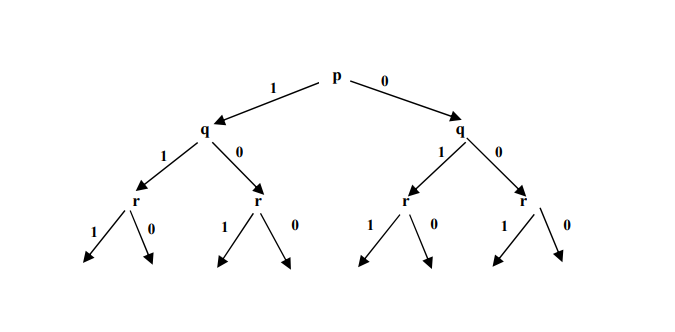
\includegraphics[width=0.8\textwidth]{Graphics/arboldp.png}
    \caption{Posible espacio de búsqueda de una FNC}
    \label{fig:arbol DP}
\end{figure}

\subsection{Davis-Putnam-Logemann-Loveland (DPLL)}
El algoritmo Davis-Putnam-Logemann-Lovelans (DPLL) aplica las mismas bases que DP, excepto que resuelve el problema de la memoria exponencial al realizar un \textit{backtrack} cronológico (al nivel anterior de decisión) en el árbol de asignaciones una vez encontrada una ``cláusula de conflicto''\footnote{Se denomina cláusula de conflicto a aquella cláusula cuyos literales evaluaron a 0 tras una asignación.}. Con este método, DPLL utiliza una estrategia \textit{``lazy''} para generar el árbol, dado que antes de ramificarse (otorgar un valor a una variable) verifica que no haya conflictos, garantizando que las asiganaciones válidas para la fórmula de entrada se encuentren en las hojas del árbol de decisión. Obsérvese que si un conflicto se produce en el nivel de decisión 0 y ambos valores para la variable ya han sido examinados, entonces se concluye que la fórmula es insatisfacible. Este proceso realizado por DPLL se denomina ramificación + propagación unitaria + retroceso.

Cabe destacar que DPLL tiene una etapa de preprocesamiento de la FNC, sobre la cual se aplican leyes de la Lógica Proposicional, así como se eliminan cláusulas redundantes mediante la aplicación de la subsunción de cláusulas\footnote{Sean $C$ y $C'$, cláusulas de una FNC; si $C' \subseteq C$, entonces se elimina $C'$ de la FNC.}. 

Obsérvese el siguiente ejemplo:

Sea la FNC:

\begin{equation*}
\{\{\neg p,\neg q\},\{\neg p, \neg q\},\{\neg p,q,\neg r\},\{\neg p,r,s\},\{p,s\}\}
\end{equation*}

Simplificando mediante la Ley de Absorción:

\begin{equation*}
\{\{\neg p,\neg q\},\{\neg p,q,\neg r\},\{\neg p,r,s\},\{p,s\}\}
\end{equation*}

Eliminando el literal puro $s$:

\begin{equation*}
\{\{\neg p,\neg q\},\{\neg p,q,\neg r\}\}
\end{equation*}

Ramificando: $p=1$

\begin{equation*}
\{\{\neg q\},\{q,\neg r\}\}
\end{equation*}

Aplicando PU:

\begin{equation*}
\{\{\neg q\},\{q,\neg r\}\}
\end{equation*}

Aplicando PU:

\begin{equation*}
\{\neg r\}
\end{equation*}

\begin{equation*}
\emptyset
\end{equation*}


Luego la FNC es satisfacible.

No obstante la reducción del espacio de memoria de DPLL respecto a DP, aún quedan problemas fundamentales: selección de variables, \textit{backtrack} cronológico y selección de cláusulas unitarias.

En primer lugar la selección de la variable a asignar un valor influye en la ``forma'' que tomará el espacio de búsqueda, por lo que malas decisiones en este sentido conllevan a caminos más largos en la búsqueda de una solución. Análogamente se gana en eficiencia considerando heurísticas en la selección de variables. (poner ejemplo)

En segundo lugar, el \textit{backtrack} cronológico a partir de un conflicto obliga a explorar el resto de las posibles asignaciones de las variables en niveles anterirores, potencialmente, de forma innecesaria, sobre todo para aquellos casos donde la asignación causante del conflicto se encuentre a $k$ niveles de distancia del nivel del conflicto. Además, DPLL no aprovecha las cláusulas que han resultado conflictos, es decir, no aprende de ellas, por lo que es vulnerable a cometer el mismo error (mismo patrón incorrecto de asignaciones para las variables involucradas en el conflicto). Esto lo hace susceptible a repetir errores de forma recurrente.

Finalmente, el problema de selección de cláusulas unitarias, influye también en la eficiencia del algoritmo. Se puede decir que guarda relacón con la estrategia de selección de variables.

\section{CDCL}
CDCL es una mejora que se le añadió al algoritmo DPLL con el objetivo de erradicar el problema del retroceso (\textit{backtrack}) cronológico, una vez encontrada una cláusula de conflicto (todos sus literales evalúan 0).

El retroceso cronológico consiste en recorrer el árbol de decisión (estructura propia del algoritmo DPLL que se forma al asignarle valores a las variables) retrocediendo de a 1 por cada nivel, probando todos los valores aún sin explorar de cada variable hasta encontrar la asignación causante del conflicto. Esta búsqueda es ineficiente dado que, además de analizar casos innecesarios, se vuelve susceptible a cometer el mismo error en el futuro (potencialmente realiza la misma combinación de asignaciones) generando búsquedas redundantes.

Para solucionar este problema, CDCL crea un grafo dirigido y acíclico que permite guardar el historial de asignaciones de cada variable. En dicho grafo, los nodos son las variables y los arcos constituyen la causa de la asignación de dicha variable: la cláusula a la que pertenece, si fue asignada por propagación unitaria, y null para variables asignadas por decisión. El grafo también contiene 2 metadatos: el valor asignado a cada variable (0 o 1), y el nivel de decisión en el que se asignó (los diferentes niveles de decisión están marcados por la asignación de valores por decisión). Cabe destacar que la dirección de los arcos en el grafo va desde las variables de decisión hacia aquellas que, en el mismo nivel, tuvieron que forzar su valor por propagación unitaria. En el caso de una nueva variable de decisión, se crea un nuevo arco con valor nulo desde la variable asignada por decisión en el nivel anterior, hasta la nueva variable.

Cuando una cláusula resulta ser de conflicto (sus literales evaluaron 0), CDCL crea un nuevo nodo en el grafo que representa dicho conflicto, para comenzar con su análisis.
Este análisis busca en el grafo la asignación causante del conflicto, para retroceder justo hacia ese punto y realizar un \textit{backjump} en lugar de un retroceso cronológico, como en DPLL. Asimismo, con este análisis CDCL busca conformar una cláusula (cláusula aprendida) que represente la combinación de asignación de valores que condujo a dicho conflicto, para incluirla en la base de datos de las cláusulas de la FNC y evitar cometer el mismo error en iteraciones futuras. El punto escogido para realizar el \textit{backjump} es conocido como primer punto de implicación único (\textit{First-UIP} por sus siglas en inglés). Este punto, será aquel literal que en la cláusula aprendida, posea el más alto nivel de decisión, diferente del actual.

Es necesario enfatizar en el hecho de que la cláusula aprendida debe contener únicamente 1 literal cuyo valor haya sido asignado en el nivel de decisión actual. En caso de haber más de uno, CDCL recorre el grafo en busca de la cláusula que causó la asignación de una de estas variables y aplica el Principio de Resolución entre esta y la cláusula aprendida hasta el momento. La cláusula resultante pasará a ser la nueva cláusula aprendida. El proceso se repetirá hasta que la cláusula aprendida contenga solo un literal cuyo valor fue asignado en el nivel de decisión actual.

En caso de que el nivel del \textit{backjump} sea el nivel 0, CDCL considera la FNC como insatisfacible.

A continuación, se muestra como ejemplo la implementación en Python de un CDCL SAT \textit{solver}

\begin{lstlisting}
class SATSolver:
    def __init__(self, formula):
        """
        Initializes the SAT solver.
        
        Parameters:
          formula: A list of clauses, where each clause is represented as a list of integers.
                   A positive integer i represents the variable x_i, and a negative integer -i represents -x_i.
        """
        # Copy the formula so that learned clauses can be appended.
        self.formula = formula[:]  
        self.assignments = {}    # Maps variable -> True/False assignment.
        self.levels = {}         # Maps variable -> decision level at which it was assigned.
        self.reasons = {}        # Maps variable -> clause that forced the assignment (None for decision variables).
        self.decision_level = 0  # Current decision level.
        self.decision_stack = [] # Stack storing tuples (variable, assigned value, decision level).

    def literal_value(self, literal):
        """
        Evaluates a literal given the current partial assignment.
        
        Returns:
          True if the literal is assigned True,
          False if the literal is assigned False,
          None if the variable is unassigned.
        """
        var = abs(literal)
        if var not in self.assignments:
            return None
        # For a positive literal, the assignment is the value; for a negative literal, invert the assignment.
        return self.assignments[var] if literal > 0 else not self.assignments[var]

    def check_clause(self, clause):
        """
        Determines the status of a clause with respect to current assignments.
        
        Returns a tuple (status, literal) where status is one of:
          - `satisfied': Clause is already True under the assignment.
          - `conflict': All literals are assigned False (the clause is unsatisfied).
          - `unit': Exactly one literal is unassigned while all others are False (this literal must be True).
          - `undefined': The clause is neither satisfied, conflicting, nor unit.
        """
        satisfied = False
        unassigned_count = 0
        unit_literal = None
        for literal in clause:
            val = self.literal_value(literal)
            if val is True:
                return (`satisfied', None)
            if val is None:
                unassigned_count += 1
                unit_literal = literal  # Last seen unassigned literal.
        if unassigned_count == 0:
            return (`conflict', None)
        if unassigned_count == 1:
            return (`unit', unit_literal)
        return (`undefined', None)

    def unit_propagate(self):
        """
        Repeatedly applies unit propagation.
        
        Returns:
          A conflicting clause if a conflict is found during propagation; otherwise, returns None.
        """
        changed = True
        while changed:
            changed = False
            for clause in self.formula:
                status, unit_literal = self.check_clause(clause)
                if status == 'conflict':
                    # A clause is unsatisfied => conflict!
                    return clause
                elif status == `unit':
                    var = abs(unit_literal)
                    if var not in self.assignments:
                        # Determine the value needed to satisfy the unit clause.
                        value = (unit_literal > 0)
                        self.assignments[var] = value
                        self.levels[var] = self.decision_level
                        self.reasons[var] = clause  # Store the clause as the reason for this assignment.
                        self.decision_stack.append((var, value, self.decision_level))
                        changed = True
        return None

    def pick_branching_variable(self):
        """
        Selects the next unassigned variable found in the formula.
        
        (In a production solver, better heuristics like VSIDS are used.)
        """
        variables = set()
        for clause in self.formula:
            for literal in clause:
                variables.add(abs(literal))
        for var in variables:
            if var not in self.assignments:
                return var
        return None

    def resolve(self, clause1, clause2, pivot):
        """
        Performs the resolution on two clauses over the pivot literal.
        
        Specifically, it returns:
          (clause1 \ {pivot}) U (clause2 \ {-pivot})
        """
        new_clause = []
        for lit in clause1:
            if lit == pivot:
                continue
            if lit not in new_clause:
                new_clause.append(lit)
        for lit in clause2:
            if lit == -pivot:
                continue
            if lit not in new_clause:
                new_clause.append(lit)
        return new_clause

    def conflict_analysis(self, conflict_clause): 
        """
        Conducts conflict analysis to find the First UIP.
        """
        learned_clause = conflict_clause.copy()
        current_level = self.decision_level

        while True:
            # Collect literals in the learned clause assigned at the current level
            current_level_lits = [
                lit for lit in learned_clause 
                if self.levels.get(abs(lit), -1) == current_level
            ]
            if len(current_level_lits) <= 1:
                break

            # Find the most recently assigned literal in current_level_lits
            last_literal = None
            # Iterate through assignments in reverse order (most recent first)
            for var, _, lvl in reversed(self.decision_stack):
                if lvl != current_level:
                    continue
                # Check if this variable is in current_level_lits
                for lit in current_level_lits:
                    if abs(lit) == var:
                        last_literal = lit
                        break
                if last_literal is not None:
                    break

            if last_literal is None:
                break  # No resolvable literals (should not happen)

            # Resolve with the reason clause of last_literal
            reason_clause = self.reasons.get(abs(last_literal))
            if reason_clause is None:
                break  # Decision literal; cannot resolve further

            learned_clause = self.resolve(learned_clause, reason_clause, last_literal)

        # Determine the backjump level
        backjump_level = 0
        for lit in learned_clause:
            lvl = self.levels.get(abs(lit), 0)
            if lvl != current_level and lvl > backjump_level:
                backjump_level = lvl

        return learned_clause, backjump_level

    def backjump(self, level):
        """
        Backtracks the search to the given decision level by undoing assignments above that level.
        """
        new_stack = []
        for var, value, lvl in self.decision_stack:
            if lvl > level:
                if var in self.assignments:
                    del self.assignments[var]
                if var in self.levels:
                    del self.levels[var]
                if var in self.reasons:
                    del self.reasons[var]
            else:
                new_stack.append((var, value, lvl))
        self.decision_stack = new_stack

    def solve(self):
        """
        The main solving loop which alternates between unit propagation, conflict analysis, and branching.
        
        Returns:
          A satisfying assignment as a dictionary mapping variables to Boolean values if the formula is SAT;
          Otherwise, returns None indicating the formula is UNSAT.
        """
        while True:
            conflict = self.unit_propagate()
            if conflict:
                if self.decision_level == 0:
                    # Conflict at level 0 indicates an unsolvable (UNSAT) condition.
                    return None
                learned_clause, backjump_level = self.conflict_analysis(conflict)
                # Learn the clause by adding it to the formula.
                self.formula.append(learned_clause)
                # Backjump to the appropriate decision level.
                self.backjump(backjump_level)
                self.decision_level = backjump_level
            else:
                var = self.pick_branching_variable()
                if var is None:
                    return self.assignments
                self.decision_level += 1
                # For this example, we simply decide that the variable is True.
                self.assignments[var] = True
                self.levels[var] = self.decision_level
                self.reasons[var] = None  # Decision assignments have no reason clause.
                self.decision_stack.append((var, True, self.decision_level))
\end{lstlisting}

La implementación anterior consiste en una clase SATSolver que realiza los pasos de CDCL dada una FNC escrita en forma de \textit{array} de \textit{arrays} donde estos últimos son las cláusulas. Por su parte, cada variable está representada por un número entero positivo y sus literales serán el propio número y su opuesto.

El primer método inicializa las estructuras con las que trabajará:
\begin{itemize}
\item \textit{assigments}: Mapea cada variable asignada con su valor.
\item \textit{levels}: Mapea cada variable aasignada con el nivel de decisión en el que se le dio su valor.
\item \textit{reasons}: Estos serán los ``arcos'' del grafo de decisión, pues mapea por cada variable asignada la cláusula que provocó su asignación, y \textit{None} para el caso de variables asignadas por decisión.
\item \textit{decision\_level}: guarda el actual nivel de decisión.
\item \textit{decision\_stack}: registra el grafo al guardar en una pila tuplas de 3 elementos: variable asignada, valor que tomó y el nivel de decisión en el que se le asignón su valor.
\end{itemize}

El bucle principal del algoritmo se encuentra en el método \textit{solve(self)} que mientras no haya conflicto asigna valores a las variables y actualiza las estructuras de la clase, y en caso de no existir más variables por asignar, entonces devuelve la solución (asignaciones para cada variable) declarando la fórmula como satisfacible. En cambio, si una cláusula conflicto es detectada y el nivel actual de decisión es 0, entonces devuelve \textit{None}, declarando no existe una asignación válida para las variables, luego la fórmula es insatisfacible.

El método encargado de realizar la propagación unitaria por cada nivel de decisión es \textit{unit\_propagate(self)}. Este, cosiste en un algoritmo de punto fijo que se ejecuta mientras haya cambio, es decir, mientras existan cláusulas unitarias, y en caso de haber una cláusula conflicto detiene el bucle y devuelve dicha cláusula. En caso de no haber conflicto, retorna \textit{None}. La salida de este algoritmo es tomada por el método \textit{solve()} explicado anteriormente. El status de una cláusula (`\textit{satisfied}', `\textit{conflict}', `\textit{unit}', `\textit{undefined}') es determinado por \textit{check\_clause(self, clause)}.

Una vez encontrada una cláusula de conflicto, se llama al método \textit{conflict\_analysis(self, conflict\_clause)}, el cual primero analiza a cuántas variables en la cláusula conflicto se le asignaron valor en el nivel de decisión actual. Esto debido a que la cláusula aprendida solo debe contener un literal cuyo valor haya sido asignado en el nivel de decisión actual. En caso de haber más de 1, se busca el último de estos literales cuya variable fue asignada, se toma a partir del grafo de decisión la cláusula que causó su asignación, y se realiza Pincipio de Resolución con esta y la actual cláusula aprendida. La cláusula resultante para a ser la cláusula aprendida hasta el momento. Este prcedimiento se repite hasta que solo quede un literal asignado en el actual nivel de decisión.

Luego de obtener la cláusula aprendida a partir de un conflicto se determina el \textit{backjump level}, el cual será el nivel de decisión más alto de los literales se la cláusula aprendida. Una vez hallado el nivel al cual retroceder, el método \textit{backjump(self, level)} realiza las actualizaciones de todas las estructuras de la clase (\textit{backjump}).


\section{DLIS}
La heurística Dynamic Largest Individual Sum (DLIS) para selección de variables, es uno de los métodos aproximados que pueden integrarse en un CDCL SAT \textit{solver} con el objetivo de aumentar la eficiencia al asignar un valor a una variable en cada nivel de decisión.

DLIS lleva un contador por cada variable que indica el número máximo que clásulas insatisfechas que pueden resolverse al asignar uno de los dos valores (0 o 1). Es decir, dada una variable $x$, se calcula la cantidad de cláusulas insatisfechas en las que aparece el literal $x$ y su complementario $\neg x$. Sea $dlis(x)$ la mayor cantidad de cláusulas que $x$ puede satisfacer, y $count_pos(x)$ y $count_neg(x)$ la cantidad de veces que aparece el literal positivo y negativo, repectivamente, en cláusulas aún sin resolver; luego:

\begin{equation*}
dlis(x)=max(count_pos(x), count_neg(x))
\end{equation*}

Teniendo en cuenta este cálcula la próxima variable a asignar será:
\begin{equation*}
x_k \mid dlis(x_k)=max(dlis(x_i)), i \in [1,n]
\end{equation*}

donde $n$ es la cantidad de variables de la FNC.

Obsétvese que si $count_pos(x_k) > count_neg(x_k)$ entonces $x_k$ tomará como valor 1, y 0 en caso contrario, puesto que el objetivo es satisfacer dichas cláusulas. Téngase en cuenta que el cálculo se le aplica a las variables que aún no han sido asignadas, además de solo tenerse en cuenta aquellos valores que aún no han sido explorados para una misma variable en el actual nivel de decisión.

La estrategia de selección de variables se puede insertar en el anterior algoritmo de CDCL en el método \textit{pick\_branching\_variable(self)} el cual se encarga de decidir la próxima variable a la cual se le asignará un valor (0 o 1). Tomando como base el código anterior y modificando el método \textit{pick\_branching\_variable(self)}, una posible implementación de DLIS podría quedar de la siguiente forma:

\begin{lstlisting}
def pick_branching_variable(self):
    """
    Selects the next unassigned variable using the DLIS heuristic.
    Returns (variable, value) to assign, or None if all variables are assigned.
    """
    pos_counts = {}
    neg_counts = {}
    # Count occurrences in unsatisfied clauses
    for clause in self.formula:
        status, _ = self.check_clause(clause)
        if status == 'satisfied':
            continue
        for lit in clause:
            var = abs(lit)
            if var not in self.assignments:
                if lit > 0:
                    pos_counts[var] = pos_counts.get(var, 0) + 1
                else:
                    neg_counts[var] = neg_counts.get(var, 0) + 1
    # Collect all variables in the formula to find unassigned ones not in any clause
    all_vars = set()
    for clause in self.formula:
        for lit in clause:
            all_vars.add(abs(lit))
    unassigned_vars = [var for var in all_vars if var not in self.assignments]
    if not unassigned_vars:
        return None
    # For variables not in pos/neg counts, set counts to 0
    for var in unassigned_vars:
        if var not in pos_counts:
            pos_counts[var] = 0
        if var not in neg_counts:
            neg_counts[var] = 0
    # Score variables based on DLIS heuristic
    scores = []
    for var in unassigned_vars:
        pos = pos_counts[var]
        neg = neg_counts[var]
        max_count = max(pos, neg)
        total = pos + neg
        scores.append((-max_count, -total, var))  # Negative for ascending sort
    scores.sort()  # Sorts by max_count (desc), then total (desc), then var (asc)
    var = scores[0][2]
    value = pos_counts[var] > neg_counts[var]
    return (var, value)

\end{lstlisting}

Las estructuras \textit{pos\_counts} y \textit{neg\_counts} almacenan la cantidad de veces que el literal positivo y el negativo, respectivamente, de una variable aparece en cláusulas aún sin satisfacer. Para actualizar estas estructuras primero se inspeccionan aquellas cláusulas que aún no han sido resueltas. Luego se completa la información con aquellas variables sin asignar que no se hayan incluido en el procedimiento anterior y se pone su contador en 0. Este puede ser el caso de variables sin asignar que solo se encuentren en cláusulas satisfechas (a otra variable de la misma cláusula se le asignó 1 como valor). Una vez actualizado el conteo por cada literal, se haya el \textit{score} por vaiable (el máximo entre ambos conteos), se ordenan de mayor a menor y se decide asignar aquella variable con el \textit{score} más alto. El valor a asignársele a esta variable es el de mayor conteo entre ambas polaridades.

Con esta estrategia DLIS busca satisfacer en una sola asignación la mayor cantidad de cláusulas posibles, sin embargo, esta estrategia resulta costosa en instancias grandes: $O(n)$ por cada nivel de decisión, donde $n$ es la cantidad de literales.

\section{VSIDS}
Por su parte, la heurística Variable State Independent Decaying Sum (VSIDS) prioriza asignarle valores aquellas variables que hayan estado en conflictos recientes. Para ello, VSIDS lleva un \textit{score} por cada literal $l$ (no por cada variable) que aumenta cada vez que aparezcan en clásulas aprendidas de conflictos. Además, para evitar que literales que hayan pertenecido a conflictos pasados y no recientes sean tenidos en cuenta por encima de los más actuales, cada cierta cantidad $T$ de conflictos se multiplica los \textit{scores} de cada literal por $\alpha$, donde $0 < \alpha < 1$ (usualmente $\alpha = 0.95$). Integrado con CDCL, VSIDS se comportaría de la siguiente forma:
\begin{enumerate}
    \item Procede el algoritmo CDCL.
    \item Si ocurre un conflicto, se añade la cláusula aprendida $\mathbf{C_{learn}}$. Luego, por cada literal $l$ tal que $l \in \mathbf{C_{learn}}$ se tiene que $score(l) += \delta$, donde $\delta$ es el incremento.
    \item Si ocurre el conflicto $T$-ésimo, entonces $\delta = \delta \cdot \alpha$ con $0 < \alpha < 1$.
    \item Si no ocurre un conflicto, se seleccionará según VSIDS la variable $v$ si $score(l_v) = \max(score(l_i))$ para todo $i$ tal que $1 \leq i \leq 2n$, con $n$ cantidad de variables. Si $l_v$ es positivo, entonces $v$ tomará valor 1, y 0 en caso contrario.
\end{enumerate}

Una posible implementación para VSIDS que se integre al código base anterior de CDCL es la siguiente.

\begin{lstlisting}
def pick_branching_variable(self):
    """
    Selects the next unassigned variable using the VSIDS heuristic (highest activity).
    """
    candidates = []
    for var in self.activity:
        if var not in self.assignments:
            candidates.append(var)
    if not candidates:
        return None
    # Select the candidate with the highest activity; in case of tie, choose the smallest variable.
    max_activity = max(self.activity[var] for var in candidates)
    best_vars = [var for var in candidates if self.activity[var] == max_activity]
    best_vars.sort()  # Deterministic tie-breaking by choosing the smallest variable
    return best_vars[0]
\end{lstlisting}

Este método solo selecciona entre las que no han sido asignadas, aquella variable con mayor \textit{score} de acuerdo al criterio de este algoritmo. Para llevarlo a cabo, se añadió a la clase \textit{SATSolver} una estructura \textit{activity} que mapea cada variable con su \textit{score}. Esta estructura se inicializaría como se muestra a continuación:

\begin{lstlisting}
# previus code
    for clause in self.formula:
        for lit in clause:
            var = abs(lit)
            if var not in self.activity:
                self.activity[var] = 0.0
\end{lstlisting}

Además, \textit{activity} se pudiese actualizar dentro del método \textit{solve(self)} de la siguiente forma:

\begin{lstlisting}
decay_factor = 0.95
while True:
           conflict = self.unit_propagate()
           if conflict:
               if self.decision_level == 0:
                    # Conflict at level 0 indicates an unsolvable (UNSAT) condition.
                   return None
               learned_clause, backjump_level = self.conflict_analysis(conflict)
               # Learn the clause by adding it to the formula.
               self.formula.append(learned_clause)
               # Update activities for variables in the learned clause
               for lit in learned_clause:
                   var = abs(lit)
                   self.activity[var] += 1.0
               # Decay all activities
               for var in self.activity:
                   self.activity[var] *= decay_factor
               # Backjump to the appropriate decision level.
               self.backjump(backjump_level)
               self.decision_level = backjump_level
# rest of code
\end{lstlisting}

\section{Reinicio (\textit{restart})}
Las estrategias de reinicio buscan no estancarse en espacios locales de búsqueda mediante un ``reinicio'' del árbol de decisión, es decir, eliminan todas las asignaciones realizadas hasta el momento y vuelven a empezar, pero manteniendo en la FNC las cláusulas aprendidas producto de CDCL, y los datos extras como \textit{scores} de los literales que hayan aportado las heurísticas de selección de variables.

Existen varios criterios para realizar los \textit{restarts}:
\begin{enumerate}
\item Fijo: se reinicia cada $k$ conflictos fijos.
\item Geométrico: cada intervalo $r_i$ crece como un secuencia geométrica de la siguiente forma: $r_0 = b; r_i = \alpha \cdot r_{i-1} \mid \alpha > 1$. Es importante definir bien el valor de $\alpha$ pues si este es muy grande los reinicios serán muy espaciados, y si es muy pequeño habrá una sobrecarga de \textit{restarts}.
\item Luby: Este reinicio se basa en la secuencia de Luby (1,1,2,1,1,2,4,1,1,2,…), obteniéndose que $r_i = b \cdot Luby(i)$, donde $r_i$ constituye el i-ésimo \textit{restart}, y $b$ es un parámetro de intervalo.
\item \textit{Glucose-style (LBD-based)}: esta estrategia está basada en el cálculo Literal Block Distance (LBD) que consiste en, dada una cláusula aprendida, contar la cantidad de niveles de decisión diferentes a los que pertenecen cada uno de sus literales. Es decir, dada una cláusula aprendida $C_{learm}$ se tiene que $LBD(C_{learn}) = \|\{level(l)\: l \in C_{learn} \}\|$. LBD busca medir la calidad de una cláusula a partir de la diversidad de niveles de decisión en una cláusula, planteando que mientras menor sea este número las variables implicadas en el conflicto estarán más cerca en el árbol de decisión, por ende más relacionadas, luego más útil la cláusula. Por tanto, a menor LBD, mayor calidad de cláusula. Ahora, la estrategia de reinicio \textit{Glucose-style} haya dos promedios de LBD para una ventana ``rápida'' (usualmente 50 o 100 últimos conflictos) y una ventana ``lenta'' (usualmente 1000 últimos confilctos)de cantidad de conflictos. Estas dos cantidades se dividen de la siguiente forma: sean $\mu_r$ promedio de LBD en la ventana rápida de últimos conflictos, y $\mu_l$ su homólogo para la ventana lenta; sea, además, $T > 1$ umbral de decisión, entonces \textit{Glucose-style} realiza la comparación $\dfrac{\mu_r}{\mu_l} > T$, y si esta resulta verdadera entonces procede con el reinicio. Esta estrategia sugiere que si el promedio de LBD en cláusulas aprendidas recientes supera significativamente al de cláusulas más antiguas, el algoritmo estaría estancado en espacios locales de búsqueda infructíferos.
\end{enumerate}

Ussando como base el código anterior de CDCL, una posible implementación para la estrategia Luby puede ser la siguiente:

\begin{lstlisting}
# restart_luby.py

from collections import deque

def luby(u, k):
    """
    Generates the k-th value of the Luby sequence multiplied by u (unit run).
    """
    def _luby(i):
        # Encuentra el mayor j tal que i = 2^j - 1
        j = 1
        while (1 << j) - 1 < i:
            j += 1
        if i == (1 << j) - 1:
            return 1 << (j - 1)
        return _luby(i - (1 << (j - 1)) + 1)
    return u * _luby(k)

class SATSolverLuby:
    def __init__(self, formula, unit_run=100):
        from restart_luby import luby  # si ejecutas desde fuera
        self.formula = formula[:]  
        self.assignments = {}
        self.levels = {}
        self.reasons = {}
        self.decision_level = 0
        self.decision_stack = []
        # Luby restart parameters
        self.unit_run = unit_run
        self.luby_idx = 1
        self.conflicts_since_restart = 0
        self.next_restart = luby(self.unit_run, self.luby_idx)

    # the same functions (literal_value, check_clause, unit_propagate,
    # pick_branching_variable, resolve, conflict_analysis, backjump)

    def solve(self):
        while True:
            conflict = self.unit_propagate()
            if conflict:
                self.conflicts_since_restart += 1
                if self.decision_level == 0:
                    return None
                learned_clause, backjump_level = self.conflict_analysis(conflict)
                self.formula.append(learned_clause)
                self.backjump(backjump_level)
                self.decision_level = backjump_level

                # restart?
                if self.conflicts_since_restart >= self.next_restart:
                    # Restart: clear assignments, preserve learned clauses
                    self.assignments.clear()
                    self.levels.clear()
                    self.reasons.clear()
                    self.decision_stack.clear()
                    self.decision_level = 0
                    # Prepare next umbral
                    self.luby_idx += 1
                    self.next_restart = luby(self.unit_run, self.luby_idx)
                    self.conflicts_since_restart = 0
            else:
                var = self.pick_branching_variable()
                if var is None:
                    return self.assignments
                self.decision_level += 1
                self.assignments[var] = True
                self.levels[var] = self.decision_level
                self.reasons[var] = None
                self.decision_stack.append((var, True, self.decision_level))
\end{lstlisting}

Análogo a las heurísticas anteriores, se añaden nuevas estructuras a la clase \textit{SATSolver}, y en base a la estrategia de \textit{restart} de Luby, se decide en el método \textit{solve(self)} si es necesario un reinicio.

De igual modo, una implementación para la estrategia \textit{Glucose-Style (LBD-based)} sería como la que se muestra a continuación:

\begin{lstlisting}
# restart_glucose.py

class SATSolverGlucose:
    def __init__(self, formula, lbd_window=50):
        self.formula = formula[:]  
        self.assignments = {}
        self.levels = {}
        self.reasons = {}
        self.decision_level = 0
        self.decision_stack = []
        # Glucose-style parameters
        self.lbd_history = []
        self.window_size = lbd_window
        self.prev_avg_lbd = float('inf')

    #same base functions: literal_value, check_clause, unit_propagate, pick_branching_variable, resolve, backjump

    def conflict_analysis(self, conflict_clause):
        learned_clause, backjump_level = super().conflict_analysis(conflict_clause)
        # Calcular LBD (Literal Block Distance)
        levels = { self.levels.get(abs(l), 0) for l in learned_clause }
        lbd = len(levels)
        # Mantener ventana de LBDs
        self.lbd_history.append(lbd)
        if len(self.lbd_history) > self.window_size:
            self.lbd_history.pop(0)
        return learned_clause, backjump_level

    def should_restart(self):
        if len(self.lbd_history) < self.window_size:
            return False
        curr_avg = sum(self.lbd_history) / len(self.lbd_history)
        # Reiniciar si la media de LBD sube respecto al ciclo anterior
        if curr_avg > self.prev_avg_lbd:
            self.prev_avg_lbd = curr_avg
            return True
        self.prev_avg_lbd = curr_avg
        return False

    def solve(self):
        while True:
            conflict = self.unit_propagate()
            if conflict:
                if self.decision_level == 0:
                    return None
                learned_clause, backjump_level = self.conflict_analysis(conflict)
                self.formula.append(learned_clause)
                self.backjump(backjump_level)
                self.decision_level = backjump_level

                # Glucose-style restart
                if self.should_restart():
                    self.assignments.clear()
                    self.levels.clear()
                    self.reasons.clear()
                    self.decision_stack.clear()
                    self.decision_level = 0

            else:
                var = self.pick_branching_variable()
                if var is None:
                    return self.assignments
                self.decision_level += 1
                self.assignments[var] = True
                self.levels[var] = self.decision_level
                self.reasons[var] = None
                self.decision_stack.append((var, True, self.decision_level))

\end{lstlisting}

\section{Selección de cláusulas unitarias}

Una de las estrategias más usadas actualmente es \textit{Two Watched Literals (TWL)}. Esta tiene por objetivo evitar el recorrido de todas las cláusulas en el momento de realizar la propagación unitaria mediante la ``vigilancia'' de dos literales $l_1$ y $l_2$ por cada cláusula. Si durante el algoritmo tanto $l_1$ como $l_2$ no han sidp evaluados, pues no es necesario revisar dicha cláusula dado que no es unitaria ni de conflicto. En cambio, si alguno ha sido asignado a 0 se busca en cada cláusula otro literal para sustituirlo y, de no ser posible implicaría que la cláusula es unitaria (asumiendo que el otro literal vigilado no tiene valor). Si ambos literales son evaluados a 0, entonces la cláusula es de conflicto. Esta estrategia reduce grandemente el costo de recorrer cada cláusula en cada nivel de asignación.

Para insertar esta estrategia en el código base de CDCL, es necesario realizar cambios en casi todos los métodos. Véase el siguiente ejemplo de implementación:

\begin{lstlisting}
import formulas as f
from collections import defaultdict, deque

class SATSolver:
    def __init__(self, formula):
        """
        Initializes the SAT solver.

        Parameters:
          formula: A list of clauses, where each clause is represented as a list of integers.
                   A positive integer i represents the variable x_i, and a negative integer -i represents -x_i.
        """
        # Copy the formula so that learned clauses can be appended.
        self.clauses = [list(c) for c in formula]
        self.assignments = {}    # Maps variable -> True/False assignment.
        self.levels = {}         # Maps variable -> decision level at which it was assigned.
        self.reasons = {}        # Maps variable -> clause that forced the assignment (None for decision vars).
        self.decision_level = 0  # Current decision level.
        self.decision_stack = [] # Stack of (variable, value, level).

        # Two-Watched Literals: map literal -> list of clause indices watching it
        self.watches = defaultdict(list)
        self._init_watches()

    def _init_watches(self):
        """Initialize two watched literals per clause."""
        for ci, clause in enumerate(self.clauses):
            # If clause has only one literal, watch it twice.
            w0 = clause[0]
            w1 = clause[1] if len(clause) > 1 else clause[0]
            self.watches[w0].append(ci)
            self.watches[w1].append(ci)

    def literal_value(self, literal):
        """
        Evaluate a literal under current partial assignment.
        Returns True, False, or None if unassigned.
        """
        var = abs(literal)
        if var not in self.assignments:
            return None
        return self.assignments[var] if literal > 0 else not self.assignments[var]

    def check_clause(self, clause):
        """
        Determine clause status: 'satisfied', 'conflict', 'unit', or 'undefined'.
        If 'unit', also return the unit literal.
        """
        unassigned = 0
        last = None
        for lit in clause:
            val = self.literal_value(lit)
            if val is True:
                return ('satisfied', None)
            if val is None:
                unassigned += 1
                last = lit
        if unassigned == 0:
            return ('conflict', None)
        if unassigned == 1:
            return ('unit', last)
        return ('undefined', None)

    def _enqueue(self, var, value, level, reason):
        """
        Assign var=value at given level with reason and push onto decision stack.
        Returns the corresponding literal for propagation.
        """
        self.assignments[var] = value
        self.levels[var] = level
        self.reasons[var] = reason
        self.decision_stack.append((var, value, level))
        return var if value else -var

    def unit_propagate(self):
        """
        Perform unit propagation using two-watched literals.
        Returns a conflicting clause if conflict, else None.
        """
        queue = deque()
        # Enqueue all literals assigned at current level
        for var, val, lvl in self.decision_stack:
            if lvl == self.decision_level:
                queue.append(var if val else -var)

        while queue:
            lit = queue.popleft()
            lit_false = -lit
            # We iterate over a snapshot since watch list may change
            watchers = list(self.watches[lit_false])
            for ci in watchers:
                clause = self.clauses[ci]
                # Try to find a new literal to watch instead of lit_false
                found_replacement = False
                for l in clause:
                    if l == lit_false:
                        continue
                    if self.literal_value(l) is not False:
                        # relocate watch from lit_false to l
                        self.watches[l].append(ci)
                        self.watches[lit_false].remove(ci)
                        found_replacement = True
                        break
                if found_replacement:
                    continue

                # No replacement found: clause must be unit or conflict
                status, unit_lit = self.check_clause(clause)
                if status == 'conflict':
                    return clause
                elif status == 'unit':
                    v = abs(unit_lit)
                    if v not in self.assignments:
                        new_lit = self._enqueue(v, unit_lit > 0, self.decision_level, clause)
                        queue.append(new_lit)
        return None

    def pick_branching_variable(self):
        """
        Select next unassigned variable (naive).
        """
        all_vars = {abs(l) for c in self.clauses for l in c}
        for v in all_vars:
            if v not in self.assignments:
                return v
        return None

    def resolve(self, c1, c2, pivot):
        """
        Resolve two clauses on pivot literal.
        Returns the resolvent.
        """
        res = [l for l in c1 if l != pivot]
        for l in c2:
            if l != -pivot and l not in res:
                res.append(l)
        return res

    def conflict_analysis(self, conflict_clause):
        """
        First-UIP conflict analysis.
        Returns (learned_clause, backjump_level).
        """
        learned = conflict_clause.copy()
        cur_lvl = self.decision_level
        while True:
            # Count lits at current level
            lvl_lits = [l for l in learned if self.levels.get(abs(l), -1) == cur_lvl]
            if len(lvl_lits) <= 1:
                break
            # Find most recent one
            last = None
            for v,_,lvl in reversed(self.decision_stack):
                if lvl != cur_lvl:
                    continue
                for l in lvl_lits:
                    if abs(l) == v:
                        last = l
                        break
                if last:
                    break
            reason = self.reasons.get(abs(last))
            if not reason:
                break
            learned = self.resolve(learned, reason, last)

        # Compute backjump level
        back_lvl = 0
        for l in learned:
            lvl = self.levels.get(abs(l), 0)
            if lvl != cur_lvl and lvl > back_lvl:
                back_lvl = lvl
        return learned, back_lvl

    def backjump(self, level):
        """
        Undo assignments above given level.
        """
        new_stack = []
        for v, val, lvl in self.decision_stack:
            if lvl > level:
                self.assignments.pop(v, None)
                self.levels.pop(v, None)
                self.reasons.pop(v, None)
            else:
                new_stack.append((v, val, lvl))
        self.decision_stack = new_stack

    def solve(self):
        """
        Main CDCL loop.
        Returns a satisfying assignment or None if UNSAT.
        """
        while True:
            conflict = self.unit_propagate()
            if conflict:
                if self.decision_level == 0:
                    return None
                learned, bj = self.conflict_analysis(conflict)
                # add learned clause and set up its watches
                self.clauses.append(learned)
                ci = len(self.clauses) - 1
                w0 = learned[0]
                w1 = learned[1] if len(learned) > 1 else learned[0]
                self.watches[w0].append(ci)
                self.watches[w1].append(ci)
                # backjump and continue
                self.backjump(bj)
                self.decision_level = bj
            else:
                var = self.pick_branching_variable()
                if var is None:
                    return self.assignments
                # make a new decision
                self.decision_level += 1
                lit = self._enqueue(var, True, self.decision_level, None)
\end{lstlisting}

En este código, de igual forma, se añaden las estrucutras necesarias y se realiza el procedimiento de acuerdo con la idea que plantea TWL.
\chapter{Propuesta}\label{chapter:proposal}

\chapter{Detalles de Implementación y Experimentos}
\label{chapter:implementation}
El objetivo de esta tesis es comparar dos de las heuristicas integradas a CDCL, en este caso, dos de las que intentan dar soluci/'on al problema de selecci/'on de variables: Dichas estrategias, VSIDS y DLIS, son comparadas usando \textit{restart} y no.

En el trabajo se usaron los lenguajes de programaci/'on C++, Python y bash. CaDiCaL est/'a programado en C++, por lo que es el lenguaje en el que est/'an implementadas las heur/'isticas. Python fue usado para automatizar los procesos de pruebas, guardar los resultados obtenidos y realizar los an/'lisis estad/'sticos. Finalemnte, bash se usa como parte de la "compilaci/'on" del solver, cuyos archivos como \textit{configure} y \textit{makefile} que vienen integrados al \textit{solver}, son los encargados de hacerlo funcionar.

\subsection{CaDiCaL}
CaDiCaL fue el \textit{solver} escogido para esta comparaci/'on, ya que cuenta con la posibilidad de activar y desactivar VSIDS (ya viene integrada), al igual que la estrategia \textit{restart}, tambi/'en integrada en el solucionador.\footnote{Cabe destacar que CaDiCaL ofrece esta misma posibilidad para much/'isimas heur/'sticas, adem/'as de estrategias para adaptar la v/'a de soluci/'on al tipo de problemas (citar documentaci/'n de CaDiCaL)} Como ya se mencion/'o con anterioridad en este documento, pr/'acticamente todos los CDCL SAT \textit{solvers} modernos no incluyen DLIS como heur/'istica de selecci/'on de variables, y CaDiCaL es uno de ellos. Por esta raz/'on, se decidi/'o integrar una implementaci/'on de DLIS a este solucionador, aprovechando la pol/'itica \textit{open source} de su c/'odigo fuente \cite{cadical2024}.%insertar link al repo original de cadical.

\subsubsection{Integraci/'on de DLIS}
Para integrar DLIS en CaDiCaL se modificaron los siguientes archivos:
\begin{itemize}
    \item \textit{internal.hpp}
    \item \textit{internal.cpp}
    \item \textit{decide.cpp}
    \item \textit{options.hpp}
\end{itemize}

{\textit{internal.hpp}}
En este archivo se declaran los m/'todos que ser/'an implementados como parte de la clase \textit{Internal} \ref{lst:cadical-dlis-internal.hpp}:

\begin{lstlisting}[
    language=C++,
    caption={Integraci\'on de DLIS en CaDiCaL. Internal.hpp},
    label={lst:cadical-dlis-internal.hpp},
    captionpos=b,
    frame=tb
]
// DLIS
int next_decision_variable_with_dlis ();
int count_literal_in_unsatisfied_binary_clauses(int lit);

\end{lstlisting}

{\textit{internal.cpp}}
En \textit{internal.cpp} se a/~nadi/'o el c/'odigo \ref{lst:cadical-dlis-logic-internal.cpp} que contiene la l/'ogica de funcionamiento de DLIS.
CaDiCaL almacena las variables de la FNC en una lista doblemente enlazada, en la que aquellas que ya han sido asignadas y las que a/'un no tienen un valor definido se encuentran separadas en dos grupos (dentro de la misma lista) separadas por un /'indice que marca el l/'mite entre ellas. Este valor va cambiando con cada asignaci/'on. Haciendo uso de esta estructura, el siguiente m/'etodo se encarga de comparar la ocurrencia, en cl/'ausulas insatisfechas, de los literales correspondientes a las variables sin asignar, y elige el de valor m/'aximo.

\begin{lstlisting}[
    language=C++,
    caption={Integraci\'on de DLIS en CaDiCaL. Internal.cpp},
    label={lst:cadical-dlis-logic-internal.cpp},
    captionpos=b,
    frame=tb
]
int Internal::next_decision_variable_with_dlis () {
  int best_lit = 0;
  int best_score = -1;

  // Empezamos en el primer nodo ``no asignado'' de la cola:
  int idx = queue.unassigned;

  // Recorremos la lista de variables sin asignar (link(idx).prev nos lleva
  // al siguiente ``sin asignar''), igual que en next_decision_variable_on_queue().
  while (idx) {
    // Si idx ya tiene val(idx) != 0, saltemos (aunque en teor\'ia queue.unassigned
    // siempre apunta a un idx tal que val(idx)==0; no obstante, por seguridad lo comprobamos).
    if (val(idx) == 0) {
      // Calcular la puntuaci\'on DLIS para +idx y para -idx
      int pos_score = count_literal_in_unsatisfied_clauses_(idx);
      int neg_score = count_literal_in_unsatisfied_clauses_(-idx);

      float med_score = (pos_score + neg_score)/2; // Se toma el promedio por la estrategia de phase

      // Comparar con el mejor hasta ahora
      if (med_score > best_score) {
        best_score = med_score;
        best_lit   = idx;    
      }      
    }
    // Avanzamos al siguiente \'indice ``no asignado'':
    idx = link(idx).prev;
  }

  LOG ("next DLIS decision literal %d with score %d", best_lit, best_score);
  return abs(best_lit);

\end{lstlisting}

Es importante aclarar que en \ref{lst:cadical-dlis-logic-internal.cpp} el c\'alculo del \textit{score} de cada literal no se hace tal cual dicta DLIS, pues en aras de mantener la consistencia del c\'odigo de CaDiCaL se usaron estrategias y estructuras que ya vienen implementadas, y a las cuales se acoplan las heur\'isticas de decisi\'on de variables que ya incorpora el solucionador. En este caso, obs\'ervese que se promedian los \textit{scores} de ambos literales. Esto, debido a que CaDiCaL implementa la estrategia \textit{phase} \ref{subsec:cadical-phasing} para elegir la polaridad de la variable. Por esta raz\'on el m\'etodo devuelve la variable y no el literal.

Obs\'ervese que este m\'etodo hace un llamado a \texttt{int count\_literal\_in\_unsatisfied\_clauses\_(idx)} que es el encargado de calcular el \textit{score} para un literal \ref{lst:cadical-dlis-calc-internal.cpp}.

\begin{lstlisting}[
    language=C++,
    caption={Integraci\'on de DLIS en CaDiCaL. Calcular \textit{score}. Internal.cpp},
    label={lst:cadical-dlis-calc-internal.cpp},
    captionpos=b,
    frame=tb
]
int Internal::count_literal_in_unsatisfied_clauses_ (int lit) {
  int count = 0;
  // Cacheamos una sola vez el valor de 'lit'.
  const signed char val_lit = val (lit);
  // Recorremos su lista de watchers
  const Watches &ws = watches (lit);
  for (const Watch &w : ws) {
    Clause *c = w.clause;                
    if (!c || c->garbage) continue;      // Saltar nulos y garbage
    int other = w.blit;                  // El otro literal de la cl\'ausula
    // Si 'lit' o 'other' ya son verdaderos, la cl\'ausula est\'a satisfecha
    if (val_lit != 0 || val (other) != 0) continue;
    ++count;
  }
  return count;
}

\end{lstlisting}

En el c\'odigo \ref{lst:cadical-dlis-calc-internal.cpp} puede verse que para efectuar el conteo de ocurrencias de un literal no se revisan todas las cl\'ausulas insatisfechas; en su lugar se aprovecha la estructura que usa CaDiCaL para aplicar la estrategia \textit{Two Watched Literals} (TWL)\ref{subsec:twl}. Luego, se recorren solo las cl\'ausulas insatisfechas donde el literal est\'e vigilado, y se procede con el c\'alculo de su \textit{score}. Con esta implementaci\'on se busca disminuir para algunos problemas el costo de recorrer todas las clausulas.

\subsubsection{\textit{decide.cpp}}
El flujo de decisi\'on sobre la pr\'oxima variable a asignar se lleva a cabo en el archivo \textit{decide.cpp}, espec\'ificamente en el siguiente m\'etodo \ref{lst:cadical-dlis-decide.cpp}:

\begin{lstlisting}[
    language=C++,
    caption={Integraci\'on de DLIS en CaDiCaL. decide.cpp},
    label={lst:cadical-dlis-decide.cpp},
    captionpos=b,
    frame=tb
]
int Internal::decide () {
  assert (!satisfied ());
  START (decide);
  int res = 0;

  //... implementacion de assumptions

    else {

    int decision = 0;
    int idx = 0;
    
    if (opts.dlis /*&& stats.decisions < threshold*/) {
      //decision = pick_dlis_branch_literal();
      idx = next_decision_variable_with_dlis ();
      LOG ("DLIS decision literal %d", decision);
    } else {
      idx = next_decision_variable ();
    }
    const bool target = (opts.target > 1 || (stable && opts.target));
    if (idx) decision = decide_phase (idx, target);
    

    if (decision) {
      stats.decisions++;
      LOG ("deciding literal %d", decision);
      search_assume_decision (decision);
    }
  }

  if (res) marked_failed = false;
  STOP (decide);
  return res;
}

\end{lstlisting}

Como se puede observar en \ref{lst:cadical-dlis-decide.cpp}, se respeta el orden de decisi\'on que sigue CaDiCaL, garantizando primero el an\'alisis de los valores de las variables seg\'un \textit{assumption} \ref{subsec:cadical-assumptions}. Luego, antes de aplicar DLIS se verifica si su flag correspondiente est\'a activada (DLIS no se usa por defecto), y en caso positivo se procede con la elecci\'on de la variable seg\'un lo explicado anteriormente. Obs\'ervese tambi\'en que heur\'isticas las heur\'sticas de decisi\'on de variables implementadas en el \textit{solver} se analizan luego de \textit{assumptions}.

Una vez escogida la variable, se llama al m\'etodo \textit{decide\_phase} para elegir su polaridad en base a la estrategia \textit{phasing} \ref{subsec:cadical-phasing}.

\subsubsection{options.hpp}
Finalmente, para habilitar la \textit{flag} \textit{--dlis=<bool>} para activar y desactivar la heur\'istica incorporada, se a\~nadi\'o la siguiente l\'inea al archivo \textit{options.hpp} \ref{lst:cadical-dlis-options.hpp}.

\begin{lstlisting}[
    language=C++,
    caption={Integraci\'on de DLIS en CaDiCaL. options.hpp},
    label={lst:cadical-dlis-options.hpp},
    captionpos=b,
    frame=tb
]
#define OPTIONS \
\
/*      NAME         DEFAULT, LO, HI,O,P,R, USAGE */ \
\
//... varias options...
OPTION( dlis,              0,  0,  1,0,0,1, "use DLIS decision heuristic") \
//...varias options...

\end{lstlisting}

\subsection{Empleo de \textit{flags} en la l/'inea de comandos}
Los \textit{flags} usados en la l/'inea de comandos para combinar las heur/'isticas fueron:
\begin{itemize}
    \item VSIDS + restart = \texttt{--score=false}
    \item VSIDS + no restart = \texttt{--score=false --restart=false}
    \item DLIS + restart = \texttt{--dlis=true --score=false}
    \item DLIS + no restart = \texttt{--dlis=true --score=false --restart=false}
\end{itemize}

La \textit{flag} \texttt{--score=false} desactiva el empleo de la estrategia EVSIDS (citar en el marco te\'orico) para usar solo el \textit{bump} caracter\'istico de VSIDS. El resto de las que est\'an son bastante descriptivas. 
Fueron usadas, adem\'as, dos \textit{flags} generales para cada heur\'istica: \texttt{-t 120} que pone un \textit{timeout} de m\'aximo 120 segundos, y \texttt{--stats} que muestra estad\'isticas extra para los problemas resueltos (resultado = \textit{SATISFIABLE}/\textit{UNSATISFIABLE}).

\subsection{Problemas}
Cada combinaci\'on de heur\'istica fue probada en cada uno de los 135 problemas generados que abarcan las siguientes categor\'ias:

\begin{itemize}
    \item Random 3-SAT 
    \begin{itemize}
        \item Se generaron 15 instancias.
        \item Tamaños de variables: 1000, 2000, 5000 (rotando cíclicamente).
        \item Relación cláusulas/variables: 3.76, 4.26 y 4.76 (alrededor del umbral de fase para 3-SAT).
        \item Ejemplo de archivo: random3sat\_n1000\_r4.26\_0.cnf.
    \end{itemize}
    \item \textit{Pigeonhole Principle} (principio del palomar)
    \begin{itemize}
        \item Se generaron 15 instancias.
        \item Número de hoyos: 10, 20, 30, 40, 50 (rotando cíclicamente).
        \item Número de palomas: siempre n\_hoyos + 1.
        \item Ejemplo de archivo: pigeon\_11\_into\_10\_0.cnf.
    \end{itemize}
    \item Random 4-SAT
    \begin{itemize}
        \item Se generaron 15 instancias.
        \item Tamaños de variables: 500, 1000, 2000 (rotando cíclicamente).
        \item Relación cláusulas/variables: 8.88, 9.88, 10.88 (alrededor del umbral de fase para 4-SAT).
        \item Ejemplo de archivo: random4sat\_n500\_r9.88\_0.cnf.
    \end{itemize}
    \item \textit{Graph Coloring} en Grafos Aleatorios
    \begin{itemize}
        \item Se generaron 10 instancias.
        \item Número de nodos: 50, 100, 200 (rotando cíclicamente).
        \item Probabilidad de arista: 0.1, 0.3, 0.5 (rotando cíclicamente).
        \item Número de colores: 3, 4, 5 (rotando cíclicamente).
        \item Ejemplo de archivo: graphcol\_n50\_p0.10\_k3\_0.cnf.
    \end{itemize}
    \item \textit{Parity} (XOR) \textit{Constraints}
    \begin{itemize}
        \item Se generaron 10 instancias.
        \item Número de variables: 10, 20, 30, 40, 50 (rotando cíclicamente).
        \item Ejemplo de archivo: parity\_n10\_0.cnf.
    \end{itemize}
    \item BMC de Flip-Flop Simple
    \begin{itemize}
        \item Se generaron 10 instancias.
        \item Profundidad del circuito: 3, 5, 7, 9, 11 (rotando cíclicamente).
        \item Ejemplo de archivo: bmc\_flipflop\_d3\_0.cnf.
    \end{itemize}
    \item Problemas \textit{DLIS-friendly}
    \begin{itemize}
        \item Se generaron 30 instancias.
        \item Número de variables: 200, 300, 400 (seleccionado aleatoriamente).
        \item Tamaño de cláusula: 5 o 6 (aleatorio).
        \item Relación cláusulas/variables: valor real entre 2.0 y 3.5 (aleatorio).
        \item Sesgo positivo en literales: entre 0.7 y 0.8 (aleatorio).
        \item Ejemplo de archivo: biased\_random5sat\_n200\_r2.45\_b0.73\_2000.cnf.
    \end{itemize}
    \item Problemas \textit{no DLIS-friendly}
    \begin{itemize}
        \item Se generaron 30 instancias.
        \item Número de variables: 1000, 2000, 5000 (aleatorio).
        \item Tamaño de cláusula: 3.
        \item Relación cláusulas/variables: valor real entre 4.0 y 5.0 (aleatorio).
        \item Sin sesgo en literales: bias\_pos = 0.5.
        \item Ejemplo de archivo: biased\_random3sat\_n1000\_r4.32\_b0.50\_3000.cnf.
    \end{itemize}
\end{itemize}


El generador cubre exhaustivamente ocho familias de problemas: Random 3-SAT, \textit{Pigeonhole}, Random 4-SAT, \textit{Graph Coloring}, \textit{Parity}, BMC Flip-Flop, \textit{DLIS-friendly} y \textit{no DLIS-friendly}. Cada familia tiene parámetros clave que varían (número de variables, relación cláusulas/variables, sesgo, tamaño de cláusula, profundidad, etc.), asegurando diversidad estructural y de dificultad en los \textit{benchmarks} generados.

\subsection{Generador de problemas}
El generador de problemas (\textit{benchmarks}) se program\'o en python y se usaron las bibliotecas \textit{os}, \textit{random} y \textit{csv}. Los resultados se exportaron a una carpeta \textit{``generated\_benchmarks''} en el mismo directorio del \textit{script} cuyos archivos se encuentran en formato DIMACS (referencia al marco te\'orico) en .cnf.

\subsection{Estad/'isticas}
El an\'alisis estad\'istico de los resultados de la comparaci\'on de cada heur\'istica por problema est\'a implementado en el archivo \textit{stats\_analysis.ipynb}. Se compar\'o los problemas cuyo resultado fue \textit{TIMEOUT} con los que s\'i resolvieron las heur\'isticas. Se hace un an\'alisis de la distribuci\'on de cada caracter\'istica en problemas \textit{TIMEOUT} por heur\'istica. Para el caso de los problemas resueltos (resultado = \textit{SATISFIABLE/UNSATISFIABLE}) se hace de igual modo un an\'alisis de la distribuci\'on y se incluye la caracter\'istica \textit{tiempo en segundos}. Posteriormente se hace un an\'alisis comparativo entre los problemasa que fueron resueltos y los que no. Para ello se realiza un an\'alisis entre variables y se eliminan aquellas que sean colineales. Esta comprobaci\'n se realiza mediante el c\'alculo del Factor de Inflaci\'on de Varianza (VIF).
Para realizar la comparaci\'on en cuanto a caracter\'isticas entre los problemas resueltos y los que no, se realizan las pruebas de Mann-Whitney U, y para visualizar los resultados se emplean gr\'aficas de caja y bigotes. Adem\'as, tambi\'en se usa regresi\'on log\'istica ya que permite interpretar c\'omo cada variable afecta la probabilidad de que ocurra o no un \textit{TIMEOUT}.

La otra parte de la evaluaci\'on consiste en un an\'alisis del rendimiento de cada combinaci\'on de heur\'isticas en cuanto al tiempo de ejecuci\'on en los problemas resueltos. Para ello se hizo un an\'alisis de la correlaci\'on de Spearman entre las caracter\'isticas de los problemas y el tiempo en segundos. Se realiz\'o, adem\'as, el test de Kruskal-Wallis para analizar si el tiempo difiere entre heur\'isticas para un mismo tipo de problema. Asimismo, se realiz\'o el test de Dunn por cada heur\'istica para realizar una comparaci\'on estad\'istica post-hoc (prueba de Dunn) para analizar si existen diferencias significativas en los tiempos de resoluci\'on (\textit{log}(\text{tiempo})) de una heur\'istica espec\'ifica en los problemas resueltos, seg\'un los valores de una caracter\'istica. 
Los resultados son graficados en \textit{boxplot}. Finalmente, se realiza una regresi\'on lineal m\'ultiple para definir qu\'e caracter\'isticas predicen el tiempo de resoluci\'on.

Para la implementaci\'on de estos an\'alisis se usaron las siguientes bibliotecas de python: \texttt{pandas}, \texttt{numpy}, \texttt{seaborn}, \texttt{matplotlib.pyplot}, \texttt{statsmodels.api}, \texttt{variance\_inflation\_factor} y variance\_inflation\_factor, ambas de \texttt{statsmodels.stats.outliers\_influence}, \texttt{ols} de \texttt{statsmodels.formula.api}, \texttt{scipy.stats}, \texttt{LogisticRegression} de \texttt{sklearn.linear\_model}, y \texttt{scikit\_posthocs.}

\section{Resultados}
\subsection{An\'alisis de los problemas con TIMEOUT}

\subsubsection{Tabla resumen de TIMEOUTs}
%Insertar referencia a tabla
En la tabla (insertar referencia) se muestran las caracteristicas de los problemas cuyo resultado fue timeout ademas del nombre de dicho problema y la heuristica. (visualizar estos datos mediante graficas)

Con base en el conjunto de resultados filtrados por TIMEOUT, se observa que las heurísticas evaluadas presentan diferencias claras en su comportamiento frente a instancias con distintas características estructurales. Por ejemplo, la heurística VSIDS combinada con reinicio tiende a experimentar TIMEOUT en instancias con menor número de variables pero con una densidad relativamente alta de cláusulas por variable, lo que sugiere que esta configuración puede ser menos efectiva en problemas más densos aunque de tamaño moderado. 

En contraste, DLIS sin reinicio acumula TIMEOUT en instancias con un mayor número de variables pero con densidad menor, indicando que esta heurística puede tener dificultades para escalar en problemas más grandes, aunque menos densos. Además, la presencia o ausencia de reinicios parece influir significativamente en el rendimiento, dado que las combinaciones con reinicio generalmente muestran un patrón distinto de TIMEOUT frente a las que no lo incorporan. 

Estas observaciones permiten suponer que la elección de heurística y estrategia de reinicio debe adaptarse a la estructura específica del problema SAT para optimizar el rendimiento y evitar fallos por límite de tiempo.

\subsubsection{Estad\'isticas descriptivas}

El análisis estadístico descriptivo y las visualizaciones mediante diagramas de caja permiten observar con mayor detalle cómo se distribuyen las características de las instancias que resultaron en TIMEOUT según la heurística aplicada. En términos generales, las cuatro heurísticas (DLIS+no-restart, DLIS+restart, VSIDS+no-restart y VSIDS+restart) presentan distribuciones muy similares en cuanto a las métricas de número de variables, número de cláusulas, densidad, tamaño promedio de cláusula y cantidad de variables positivas y negativas.

Por ejemplo, en la figura \ref{fig:num-vars-timeout-x-heuristica} puede apreciarse que el número de variables en los casos con TIMEOUT oscila entre valores mínimos cercanos a 100 y máximos de 5000, con medianas alrededor de 2000 para todas las heurísticas, lo que indica que los problemas que causan TIMEOUT no se limitan a un rango estrecho de tamaño.

\begin{figure}[ht]
    \centering
    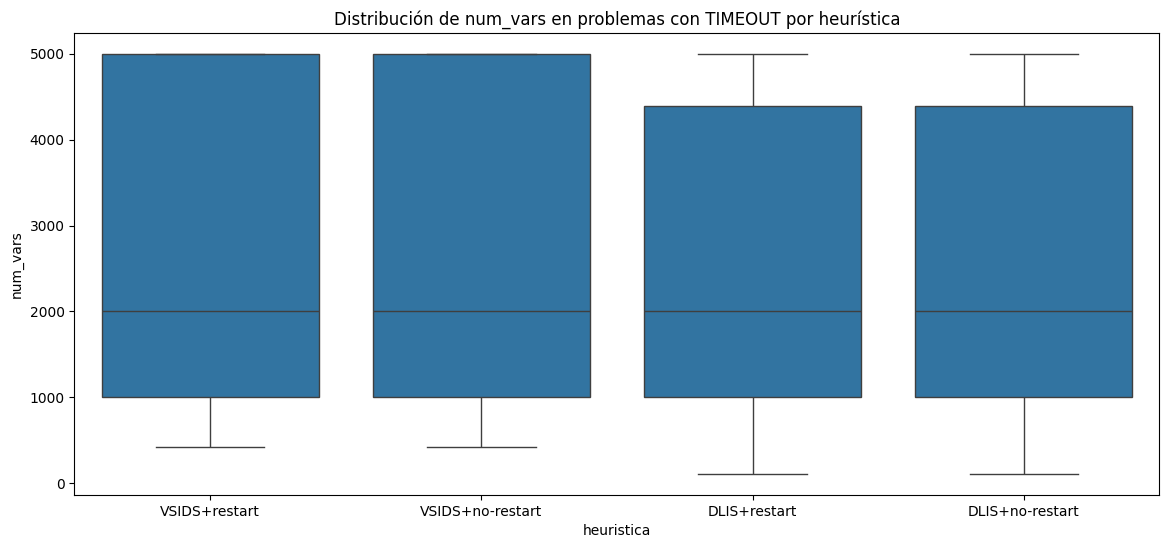
\includegraphics[width=0.8\textwidth]{Graphics/num_vars_timeout_x_heuristica.png}
    \caption{Distribuci\'on de n\'umero de variables en problemas con timeout por heur\'istica.}
    \label{fig:num-vars-timeout-x-heuristica}
\end{figure}

Por otro lado, en la figura \ref{fig:num-claus-timeout-x-heuristica} puede observarse que el n\'umero de cl\'ausulas de las instancias analizadas muestra valores elevados y gran variabilidad, con promedios entre 15.758 y 16.875 cl\'ausulas y m\'aximos por encima de 63.000. No se observan diferencias significativas entre las estrategias con DLIS o VSIDS, ni tampoco al incorporar o no el mecanismo de restart.

\begin{figure}[ht]
    \centering
    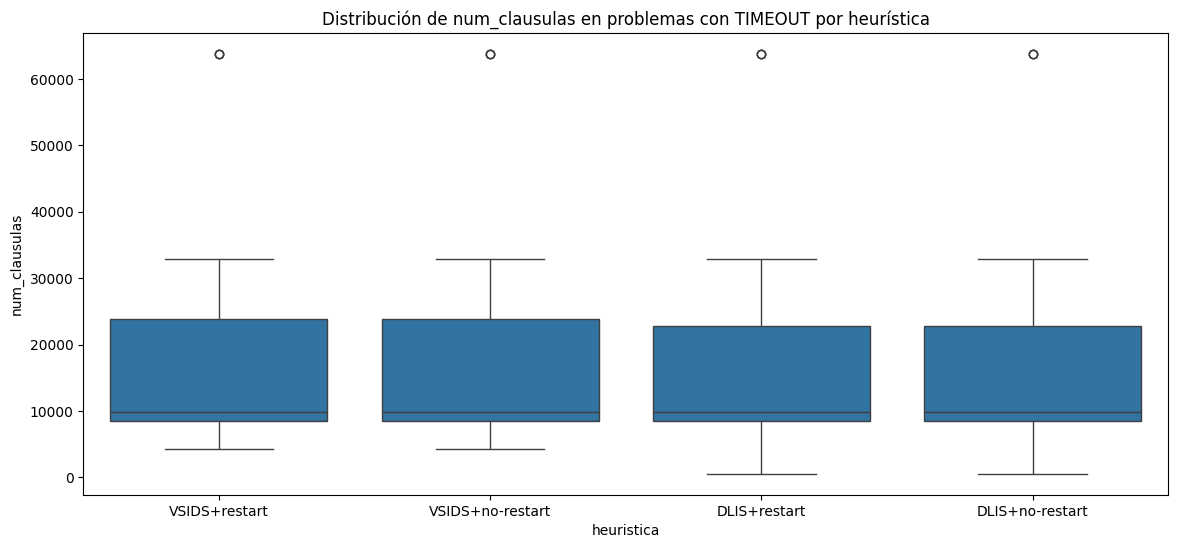
\includegraphics[width=0.8\textwidth]{Graphics/num_claus_timeout_x_heuristica.png}
    \caption{Distribuci\'on de n\'umero de cl\'ausulas en problemas con timeout por heur\'istica.}
    \label{fig:num-claus-timeout-x-heuristica}
\end{figure}

Como se muestra en \ref{fig:densidad-timeout-x-heuristica}, la densidad media se mantiene cercana a 7.4–7.7 para todas las heurísticas, con una dispersión considerable que alcanza hasta 25, lo que refleja que tanto problemas poco densos como muy densos pueden provocar fallos por tiempo.

\begin{figure}[ht]
    \centering
    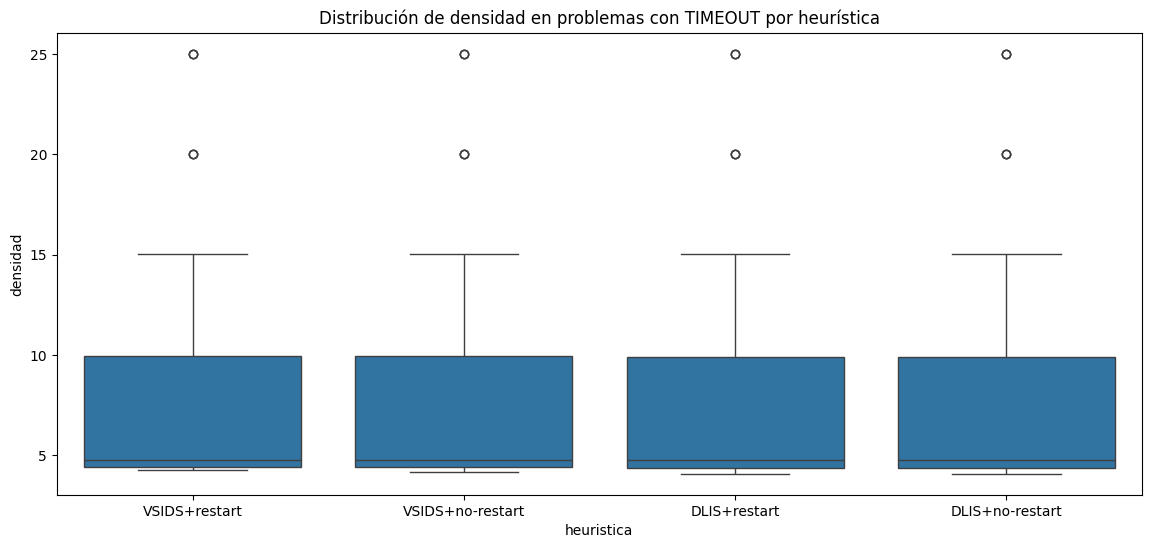
\includegraphics[width=0.8\textwidth]{Graphics/densidad_timeout_x_heuristica.png}
    \caption{Distribuci\'on de densidad en problemas con timeout por heur\'istica.}
    \label{fig:densidad-timeout-x-heuristica}
\end{figure}

En la figura \ref{fig:tamanio-prom-claus-timeout-x-heuristica} se puede apreciar que el tamaño promedio de cláusula se mantiene estable alrededor de 3, con poca variabilidad, sugiriendo que esta característica no discrimina el comportamiento de las heurísticas en cuanto a TIMEOUT.

\begin{figure}[ht]
    \centering
    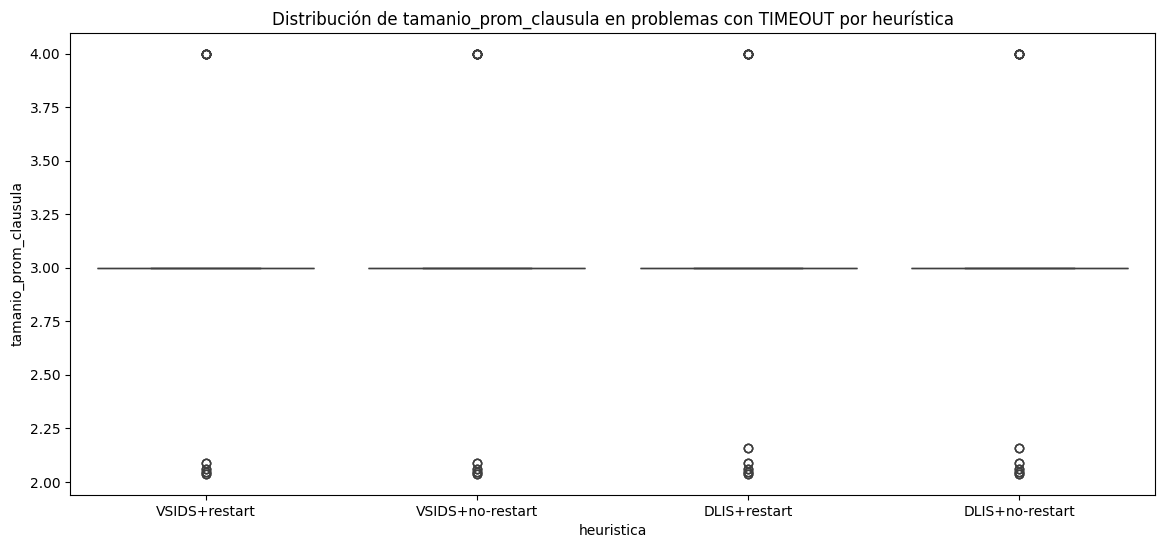
\includegraphics[width=0.8\textwidth]{Graphics/tamanio_prom_claus_timeout_x_heuristica.png}
    \caption{Distribuci\'on de tama\~no promedio de cl\'ausula en problemas con timeout por heur\'istica.}
    \label{fig:tamanio-prom-claus-timeout-x-heuristica}
\end{figure}

Por su parte, en las gr\'aficas \ref{fig:vars-pos-timeout-x-heuristica} y \ref{fig:vars-neg-timeout-x-heuristica}, se puede ver que las variables positivas y negativas, respectivamente, también muestran simetría y valores medios similares entre heurísticas, lo que implica que la polaridad de las variables no es un factor determinante en la ocurrencia de TIMEOUT.

\begin{figure}[ht]
    \centering
    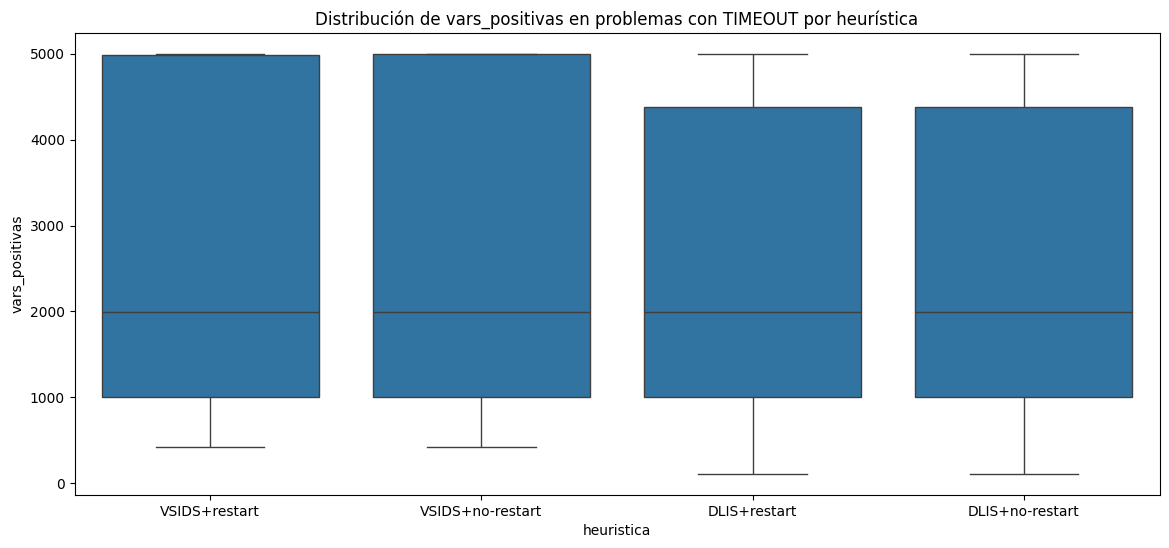
\includegraphics[width=0.8\textwidth]{Graphics/vars_pos_timeout_x_heuristica.png}
    \caption{Distribuci\'on de variables positivas en problemas con timeout por heur\'istica.}
    \label{fig:vars-pos-timeout-x-heuristica}
\end{figure}

\begin{figure}[ht]
    \centering
    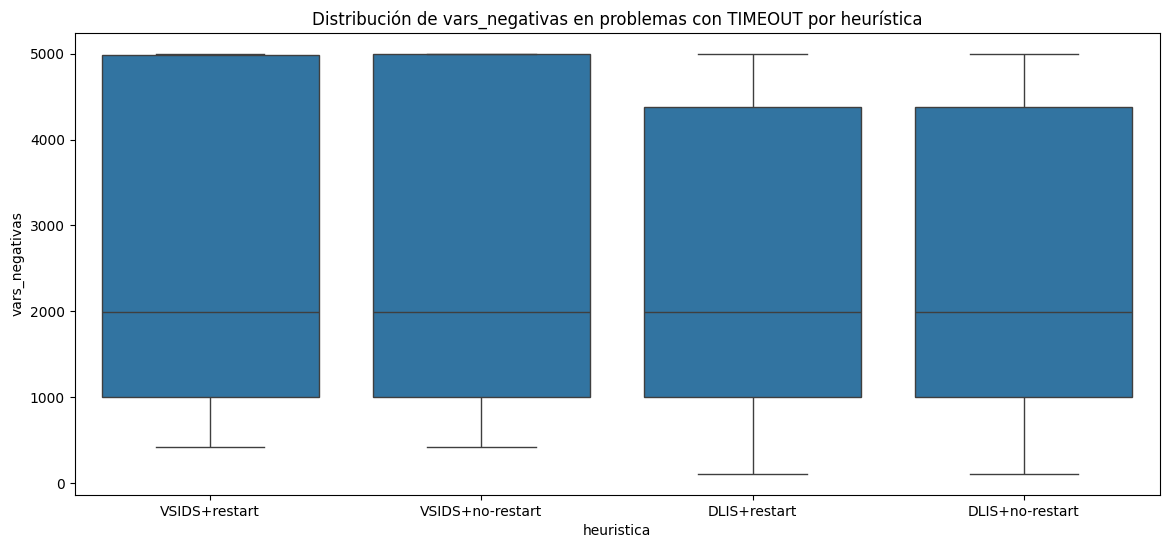
\includegraphics[width=0.8\textwidth]{Graphics/vars_neg_timeout_x_heuristica.png}
    \caption{Distribuci\'on de variables negativas en problemas con timeout por heur\'istica.}
    \label{fig:vars-neg-timeout-x-heuristica}
\end{figure}

En conjunto, estos resultados sugieren que las diferencias en el rendimiento entre heurísticas no se explican fácilmente por las características básicas de las instancias con TIMEOUT.

Las visualizaciones de caja muestran solapamientos amplios en las distribuciones de cada caracter\'istica por heur\'istica.

\subsubsection{Conteo de TIMEOUT por heur\'istica y por problema}

En las gr\'aficas \ref{fig:timeouts-x-heuristica} y \ref{fig:timeouts-x-problema} se puede observar que los problemas que tomaron mas tiempo en resolverse coinciden con los los planteados en la literatura que resultan mas dificiles de resolver a instancias SAT. Respecto a la cantidad de problemas con TIMEOUTS por heuristica, se puede apreciar que DLIS, independientemente del restart, se comporta mas lento que vsids para algunos problemas. Por su parte, vsids con restart se comporta mas lento que vsids sin restart para unas pocas instancias.

\begin{figure}[ht]
    \centering
    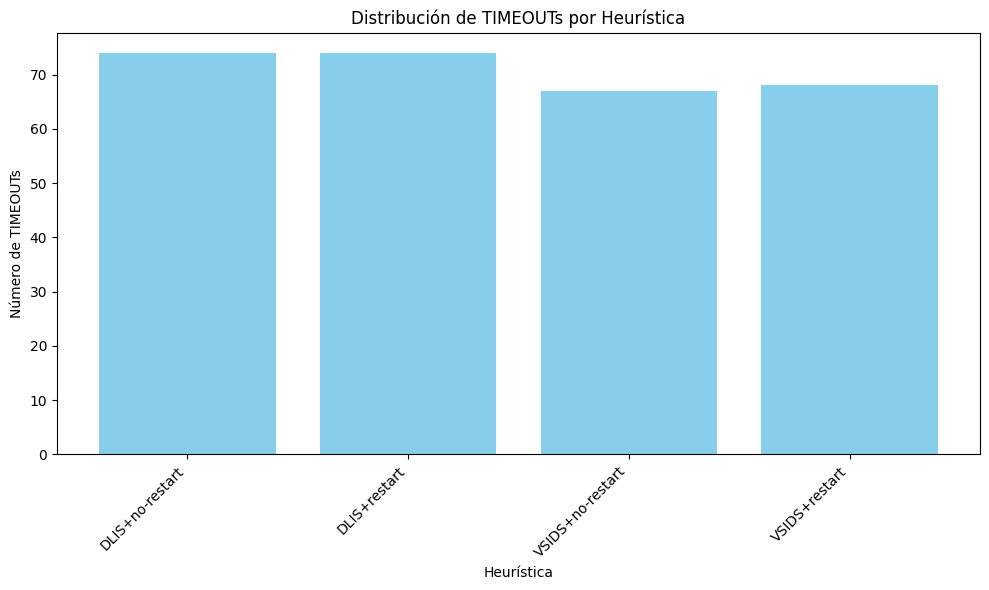
\includegraphics[width=0.8\textwidth]{Graphics/timeouts_x_heuristica.png}
    \caption{Distribuci\'on de timeouts por heur\'istica.}
    \label{fig:timeouts-x-heuristica}
\end{figure}

\begin{figure}[ht]
    \centering
    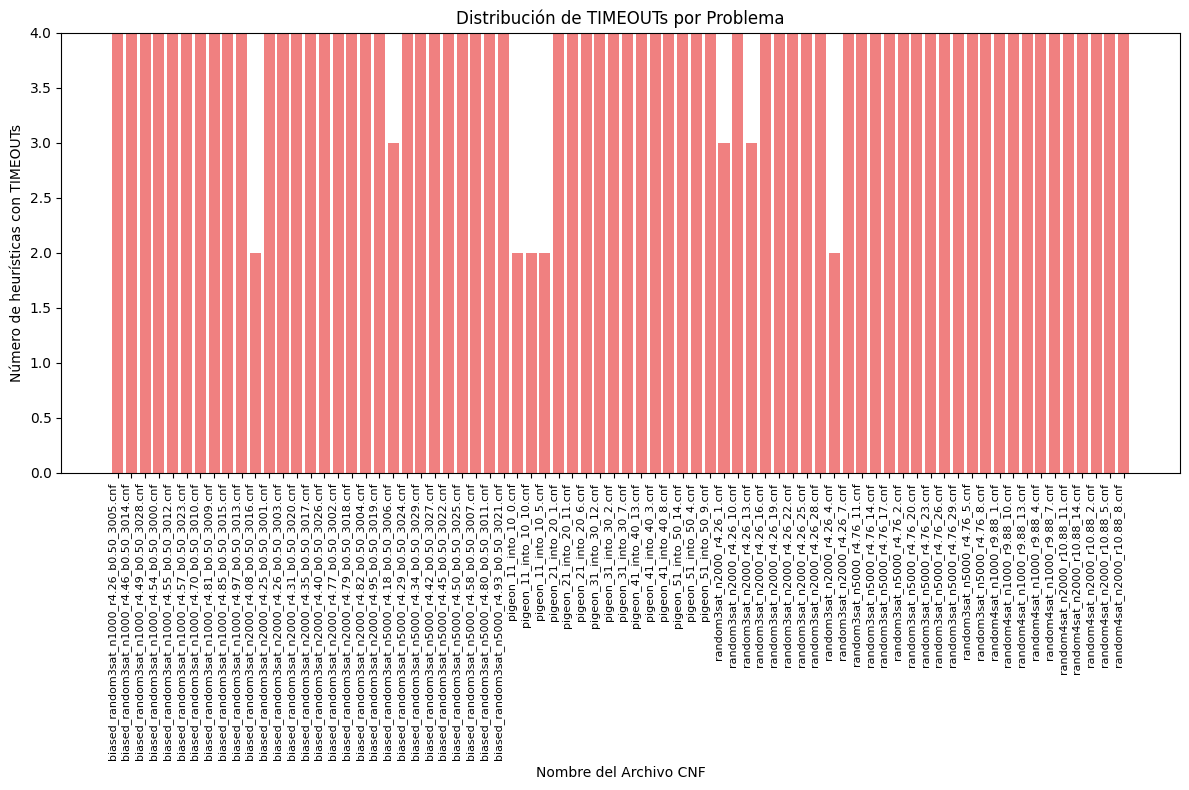
\includegraphics[width=0.8\textwidth]{Graphics/timeouts_x_problema.png}
    \caption{Distribuci\'on de timeouts por problema.}
    \label{fig:timeouts-x-problema}
\end{figure}

\subsection{An\'alisis de problemas resueltos (SATISFIABLE/UNSATISFIABLE)}

\subsubsection{Tabla resumen de RESUELTOS}
(insertar grafico que describa los resultados de la tabla filtrada por problemas resueltos)

El análisis de los problemas resueltos muestra que las instancias que concluyeron satisfactoriamente (ya sea SATISFIABLE o UNSATISFIABLE) abarcan un amplio rango de tamaños y características, desde problemas muy pequeños con 6 variables y 12 cláusulas hasta otros considerablemente más grandes con hasta 5000 variables y más de 23000 cláusulas.

Los tiempos de resolución registrados varían notablemente, desde fracciones de segundo en problemas pequeños (por ejemplo, alrededor de 0.0014 segundos en instancias con 6 variables) hasta varios segundos en problemas más complejos (por ejemplo, cerca de 9 segundos en instancias con 500 variables y alta densidad). Esto indica que, aunque el solver puede resolver eficientemente instancias pequeñas o medianas, el tiempo de cómputo crece conforme aumentan la cantidad de variables y cláusulas, así como la densidad del problema.

La presencia de las cuatro heurísticas en los resultados resueltos sugiere que todas son capaces de resolver ciertos conjuntos de problemas. Sin embargo, la diversidad en tiempos y tamaños sugiere que la heurística y la estrategia de reinicio podrían influir en la eficiencia, especialmente en problemas de mayor escala.

\subsubsection{Estad\'isticas descriptivas}


El análisis estadístico descriptivo del tiempo de resolución y las características de las instancias resueltas por cada heurística revela patrones importantes sobre el comportamiento del \textit{solver}. Estos resultados pueden apreciarse en conjunto en la gr\'afica \ref{fig:caract-tiempo-x-heuristica}.

\begin{figure}[ht]
    \centering
    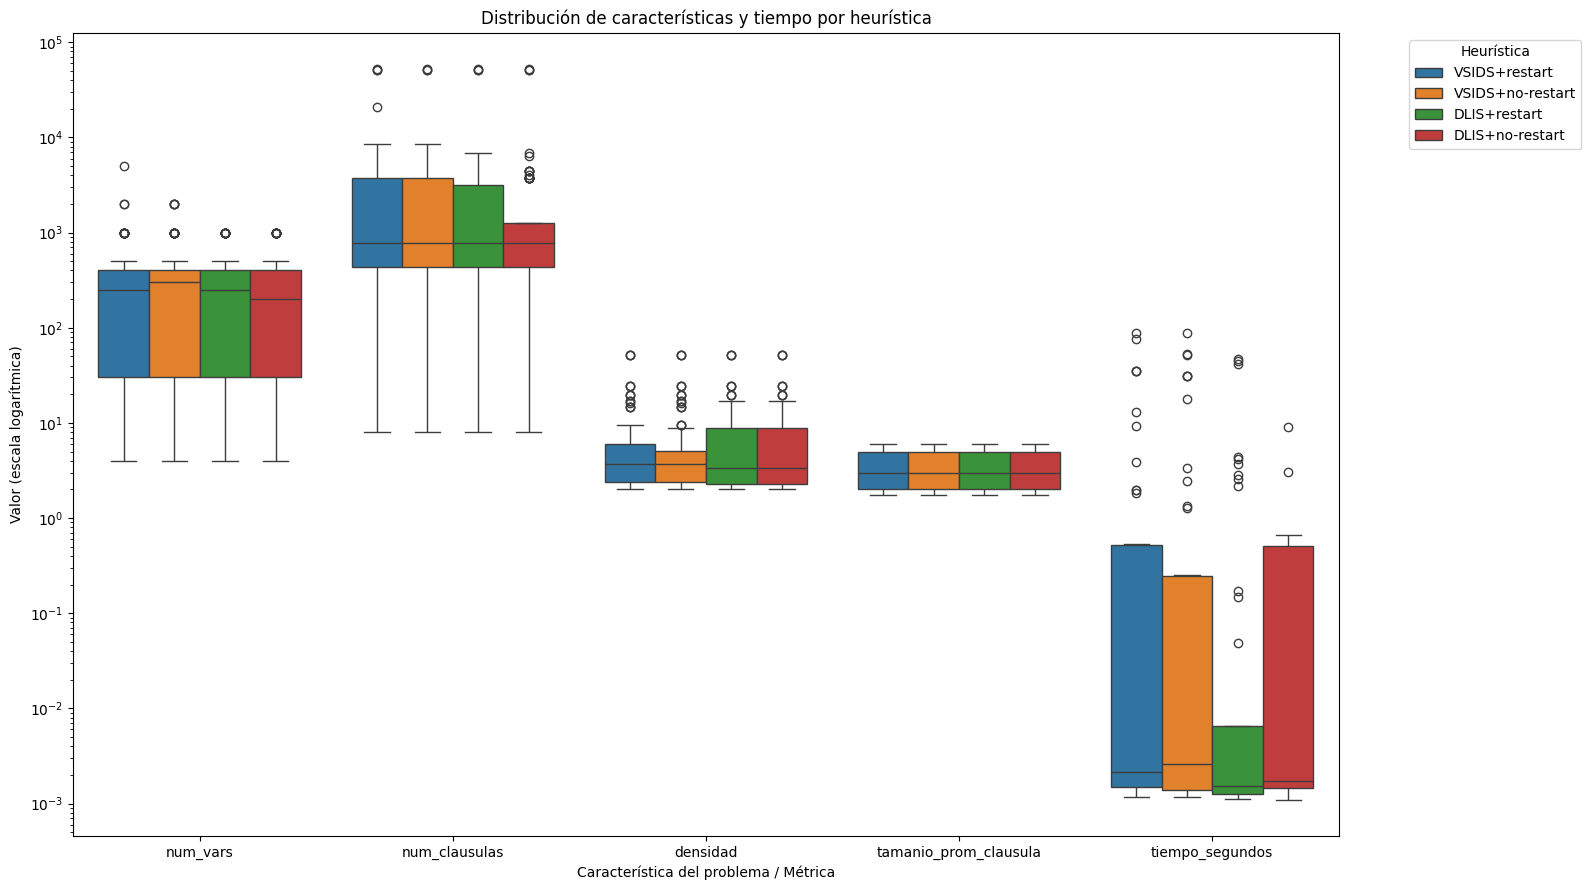
\includegraphics[width=0.8\textwidth]{Graphics/caracteristica_tiempo_x_heuristica.png}
    \caption{Distribuci\'on de caracter\'isticas y tiempo por heur\'istica.}
    \label{fig:caract-tiempo-x-heuristica}
\end{figure}


En primer lugar, se observa que las instancias resueltas por las cuatro heurísticas (DLIS+no-restart, DLIS+restart, VSIDS+no-restart y VSIDS+restart) cubren un rango amplio en tamaño, con número de variables promedio entre 322 y 403, y máximos que alcanzan hasta 2000 o incluso 5000 variables en el caso de VSIDS+restart. La cantidad de cláusulas también presenta gran dispersión, con medias cercanas a 3100–3400 y máximos que superan las 50,000, lo que indica que el solver puede manejar problemas desde muy pequeños hasta instancias complejas. La densidad promedio se mantiene alrededor de 7,2 a 7,4, con valores máximos muy altos (hasta 51.9), reflejando diversidad en la estructura de los problemas.

En cuanto al tiempo de resolución, se evidencia una marcada diferencia entre heurísticas: DLIS+no-restart presenta el tiempo medio más bajo (~0.37 s), seguido por DLIS+restart (~3.13 s), mientras que VSIDS+no-restart y VSIDS+restart muestran tiempos medios más elevados, cerca de 4.98 y 4.98 segundos respectivamente, con alta variabilidad (desviaciones estándar muy grandes y máximos que superan los 80 segundos). Esta dispersión sugiere que aunque VSIDS puede ser eficiente en muchos casos, también enfrenta problemas que requieren tiempos significativamente mayores. Además, la mediana del tiempo para todas las heurísticas es muy baja (en el orden de milisegundos), indicando que la mayoría de las instancias se resuelven rápidamente, pero existen casos atípicos que prolongan el tiempo promedio.

El tamaño promedio de cláusula es similar entre heurísticas, alrededor de 3.4, y las variables positivas y negativas mantienen valores simétricos, lo que indica que estas características no explican las diferencias en tiempo.

En conjunto, estos resultados sugieren que la elección de heurística impacta significativamente el tiempo de resolución en ciertos problemas, especialmente en instancias grandes o complejas, y que VSIDS puede tener mayor variabilidad en rendimiento.

\subsection{Porblemas RESUELTOS vs TIMEOUT}

\subsubsection{An\'alisis de multicolinealidad}

\begin{figure}[ht]
    \centering
    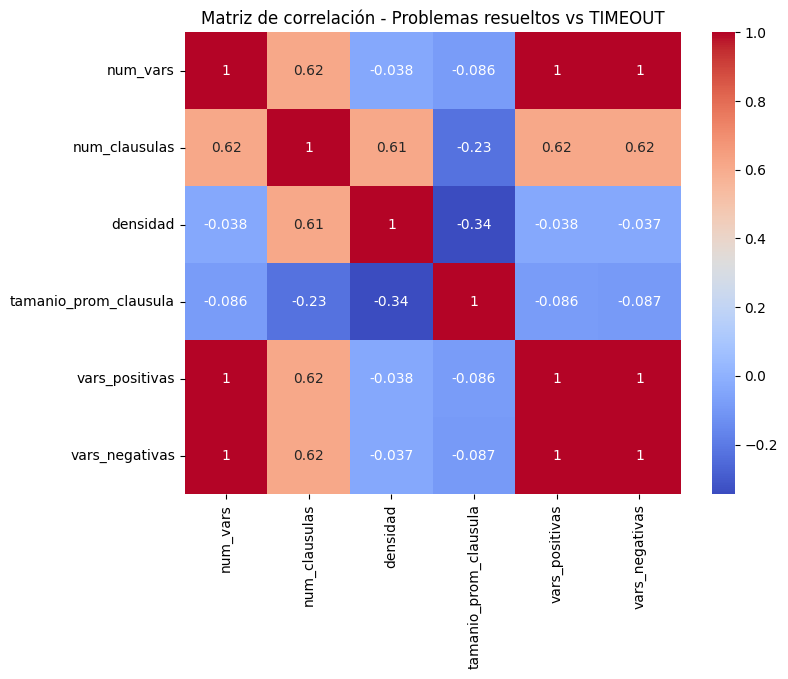
\includegraphics[width=0.8\textwidth]{Graphics/correlation_matrix_solveds_vs_timeouts.png}
    \caption{Matriz de correlaci\'on - Problemas resueltos vs TIMEOUTS.}
    \label{fig:correlation-matrix-solved-vs-timeout}
\end{figure}

Como se puede apreciar en la matriz de correlaci\'on \ref{fig:correlation-matrix-solved-vs-timeout}, entre las variables num\_vars y vars\_positivas y vars\_negativas, existe correlaci\'on perfecta ($r=1$). Adem\'as, existe una correlaci\'on moderada entre las variables num\_clausulas con vars\_negativas, vars\_positivas, num\_vars y densidad). Luego, es necesario reducir el conjunto de caracter\'isticas, quedando  el siguiente: \texttt{caracteristicas\_reducidas = ['num\_vars', 'densidad', 'tamanio\_prom\_clausula']}.

\begin{figure}[ht]
    \centering
    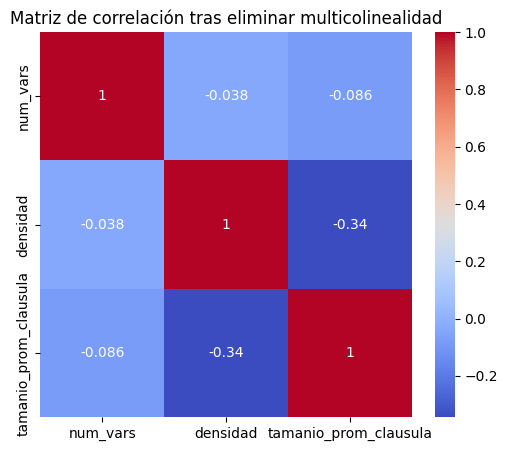
\includegraphics[width=0.8\textwidth]{Graphics/correlation_matrix_after_delete_multicol.png}
    \caption{Matriz de correlaci\'on tras eliminar multicolinealidad.}
    \label{fig:correlation-matrix-after-delete-multicol}
\end{figure}

Como se muestra en la matriz \ref{fig:correlation-matrix-after-delete-multicol}, se elimin\'o las correlaciones moderadas y severas.

\subsubsection{Comparaci\'on de caracter\'isticas entre RESUELTOS Y TIMEOUTs}

Al realizar el test de normalidad de Shapiro-Wilk se obtuvo los resultados mostrados en \ref{fig:test-shapiro-wilk}:


\begin{figure}[ht]
    \centering
    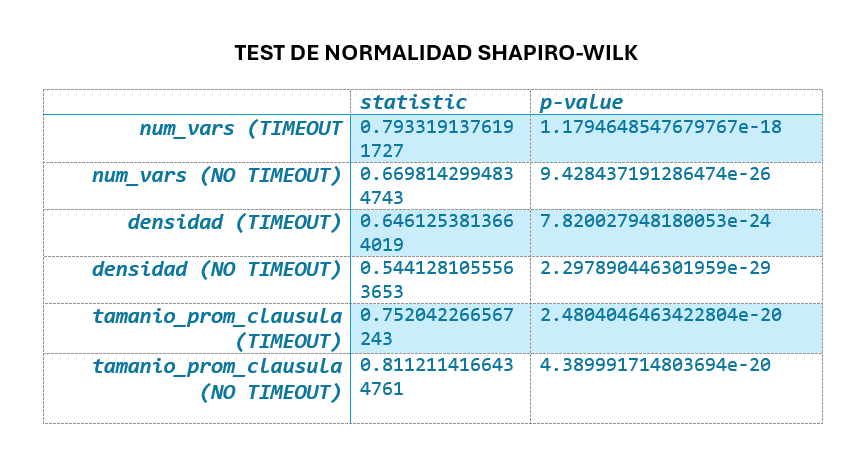
\includegraphics[width=0.8\textwidth]{Graphics/test_shapiro_wilk.png}
    \caption{Test de normalidad Shapiro-Wilk.}
    \label{fig:test-shapiro-wilk}
\end{figure}

Este an\'alisis mostrado en la tabla \ref{fig:test-shapiro-wilk} revela que ninguna de estas características sigue una distribución normal en los grupos de instancias que terminaron en TIMEOUT ni en las que fueron resueltas. Esto se evidencia en los valores de p muy bajos (todos menores a 0.05, incluso extremadamente cercanos a cero), lo que permite rechazar la hipótesis nula de normalidad para cada variable en ambos grupos. En concreto, los estadísticos de Shapiro oscilan entre aproximadamente 0.54 y 0.81, y los p-valores indican una desviación significativa de la normalidad.

Luego, para comparar estas características entre instancias con y sin TIMEOUT no es apropiado utilizar pruebas paramétricas basadas en la normalidad, como el t-test, sino que se deben emplear métodos no paramétricos, por ejemplo la prueba de Mann-Whitney, cuyo resultado se presenta a continuaci\'on. 

\subsubsection{Prueba Mann-Whitney U}

\begin{figure}[ht]
    \centering
    
\includegraphics[width=0.8\textwidth]{Graphics/prueba_mann_whitney_u.png}
    \caption{Prueba Mann-Whitney U.}
    \label{fig:prueba-mann-whitney-u}
\end{figure}

Como se muestra en \ref{fig:prueba-mann-whitney-u}, la prueba muestra resultados concluyentes sobre las diferencias entre las instancias que terminaron en TIMEOUT y las que fueron resueltas. Estos, visualizarse de igual forma mediante las gr\'aficas \ref{fig:dist-man-whitney}.


\begin{figure}[ht]
    \centering
    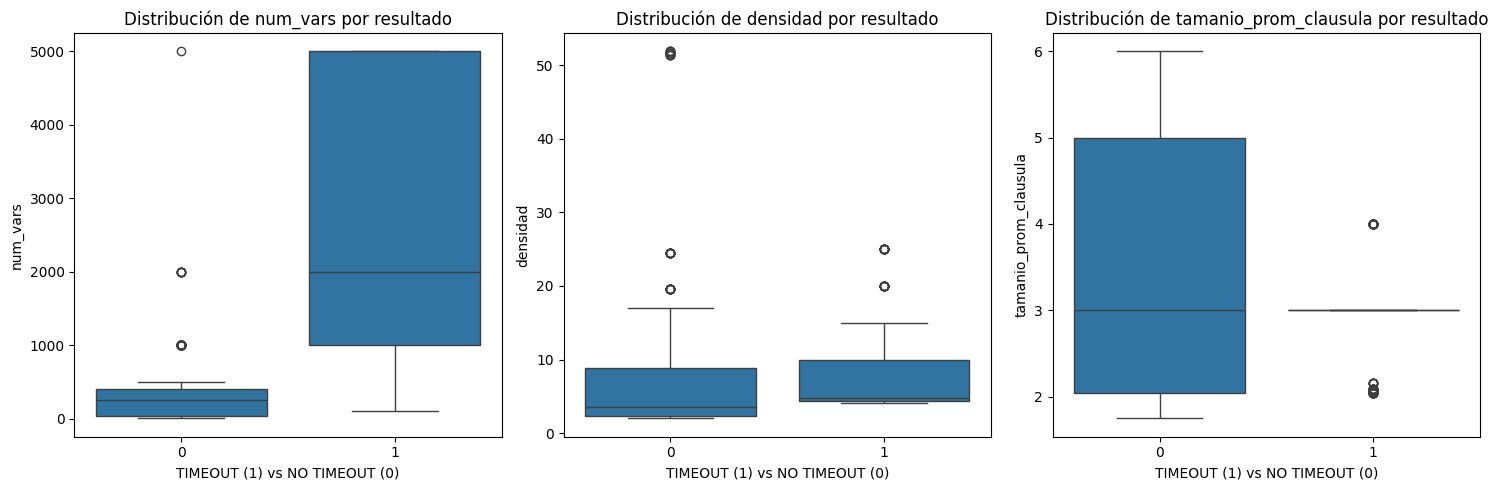
\includegraphics[width=0.8\textwidth]{Graphics/man_whitney.png}
    \caption{Distribuciones de prueba Mann-Whitney U por resultados.}
    \label{fig:dist-man-whitney}
\end{figure}

Para las variables n\'umero de variables y densidad, los valores p son extremadamente bajos (1.383e-83 y 3.168e-29 respectivamente), lo que indica diferencias estadísticamente significativas entre ambos grupos en estas características. Esto sugiere que tanto el tamaño del problema como su densidad influyen fuertemente en la probabilidad de que un problema termine en TIMEOUT.

En contraste, para el tamaño promedio de cláusula el p-valor es alto (0.803), lo que implica que no hay evidencia suficiente para afirmar que esta característica difiera entre problemas con y sin TIMEOUT.

Estos resultados confirman que las variables relacionadas con la escala y complejidad estructural del problema (num\_vars y densidad) son factores determinantes en el rendimiento del \textit{solver}, mientras que el tamaño promedio de las cl\'ausulas no parece ser un factor discriminante en la ocurrencia de TIMEOUT.

En consecuencia, para modelar o predecir la probabilidad de TIMEOUT conviene priorizar las variables num\_vars y densidad, y descartar o tratar con menor peso el tamaño promedio de cláusula.

\subsubsection{Regresi\'on log\'istica: ¿Qué caracter\'isticas predicen TIMEOUT?}

Trasa efectuar la regresi\'on se obtuvieron los siguientes resultados \ref{fig:regresion-logistica}:

\begin{figure}[ht]
    \centering
    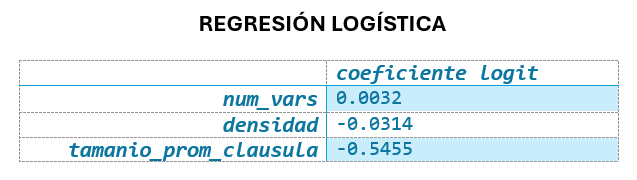
\includegraphics[width=0.8\textwidth]{Graphics/regresion_logistica.png}
    \caption{Regresi\'on log\'istica.}
    \label{fig:regresion-logistica}
\end{figure}

Con base en estos resultados de la tabla \ref{fig:regresion-logistica} , el modelo ofrece una interpretación clara sobre la influencia de cada característica en la probabilidad de que un problema no se resuelva en el tiempo límite.

El coeficiente positivo para num\_vars (0.0032) indica que a medida que aumenta el número de variables, la probabilidad de TIMEOUT también incrementa, lo cual es consistente con la intuición y los análisis descriptivos previos que mostraron que problemas más grandes tienden a ser más difíciles de resolver. 

Por otro lado, los coeficientes negativos para densidad (-0.0314) y especialmente para tamaño promedio de cláusula (-0.5455) sugieren que, manteniendo constante el número de variables, un aumento en estas características está asociado con una menor probabilidad de TIMEOUT. En particular, el tamaño promedio de cláusula tiene un efecto considerablemente más fuerte en sentido negativo, lo que podría indicar que cláusulas más largas o complejas, dentro del rango observado, facilitan la resolución o están asociadas a problemas menos propensos a agotar el tiempo.

Estos signos y magnitudes reflejan que la complejidad estructural del problema no se reduce solo al tamaño, sino que la forma en que las cláusulas están construidas también impacta el rendimiento del solver. En conjunto, el modelo confirma y cuantifica las tendencias observadas en análisis estadísticos previos, y ofrece una base para predecir y ajustar heurísticas en función de las características del problema para minimizar la ocurrencia de TIMEOUT.

\subsection{Rendimiento de las heur\'isticas en problemas resueltos}
Para los an\'alisis estad\'isticos en esta secci\'on se incluy\'o la variable tiempo, que e=indica en seg cu\'anto tard\'o el \textit{solver} en dar una soluci\'on.

\subsubsection{Correlaci\'on de Spearman}
Se obtuvo los siguientes resultados \ref{fig:correlacion-spearman}:

\begin{figure}[ht]
    \centering
    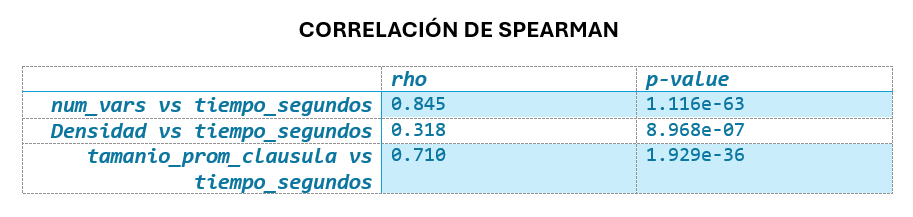
\includegraphics[width=0.8\textwidth]{Graphics/correlacion_spearman.png}
    \caption{Correlaci\'on de Spearman.}
    \label{fig:correlacion-spearman}
\end{figure}

Los resultados que se muestran en la tabla \ref{fig:correlacion-spearman} an\'alisis revela asociaciones significativas y de distinta intensidad.

La variable número de variables muestra una correlación muy fuerte y positiva con el tiempo de resolución (rho = 0.845, p < 0.001), indicando que a mayor tamaño del problema, mayor es el tiempo requerido para resolverlo, lo cual es coherente con la complejidad esperada en problemas SAT.

La densidad presenta una correlación positiva moderada (rho = 0.318, p < 0.001), lo que sugiere que problemas con mayor densidad de cláusulas por variable tienden a requerir más tiempo, aunque este efecto es menos pronunciado que el del tamaño.

Por último, el tamaño promedio de cl\'ausula tambi\'en exhibe una correlación fuerte positiva (rho = 0.710, p < 0.001), indicando que cláusulas más largas o complejas están asociadas con un aumento significativo en el tiempo de resolución.

Estos resultados confirman que tanto la escala del problema como su estructura influyen en el rendimiento del solver, siendo el número de variables el factor más determinante, seguido por la complejidad de las cláusulas y la densidad. 

\subsubsection{Kruskal-Wallis: ¿El tiempo difiere entre heurísticas para un mismo tipo de problema?}


\begin{figure}[ht]
    \centering
    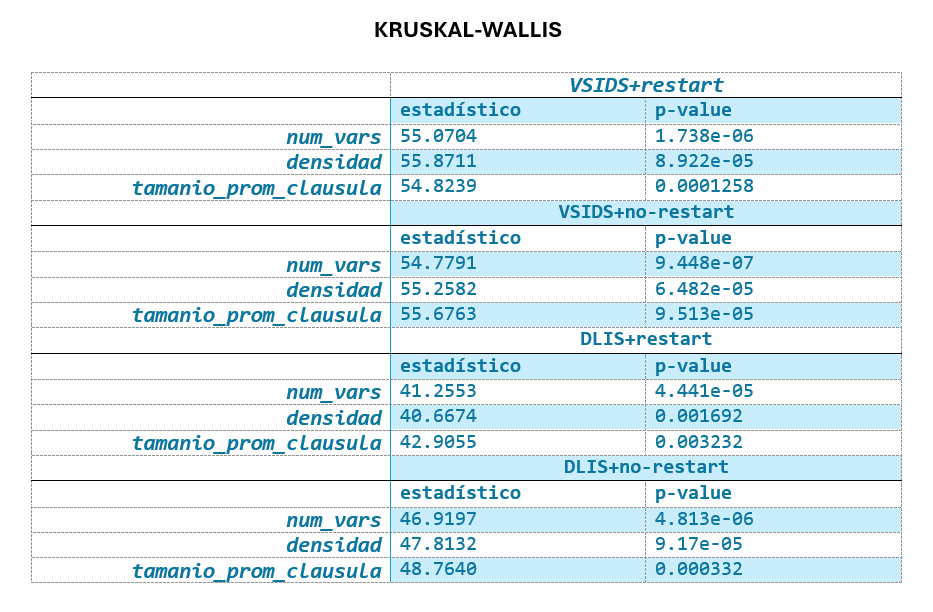
\includegraphics[width=0.8\textwidth]{Graphics/kruskal_wallis.png}
    \caption{Kruskal-Wallis.}
    \label{fig:kruskal-wallis}
\end{figure}


Dados los siguientes resultados mostrados en la tabla \ref{fig:kruskal-wallis}, se tiene que el análisis mediante la prueba no paramétrica de Kruskal-Wallis aplicado a la variable transformada del tiempo de resolución (logaritmo natural del tiempo más uno) para cada heurística y característica del problema revela diferencias estadísticamente significativas en todos los casos evaluados.

Para las cuatro heurísticas (VSIDS+restart, VSIDS+no-restart, DLIS+restart y DLIS+no-restart), las variables número de variables, densidad y tamaño promedio de cláusula muestran valores de estadístico elevados y p-valores muy bajos (todos menores a 0.005), lo que indica que la distribución del tiempo de resolución difiere significativamente entre los distintos grupos definidos por cada una de estas características. Esto implica que, independientemente de la heurística utilizada, las propiedades estructurales del problema impactan de forma relevante en el rendimiento temporal del \textit{solver}.

La consistencia de estos resultados a través de todas las heurísticas sugiere que la influencia de estas variables es robusta y generalizable, reafirmando su importancia en el análisis y modelado del comportamiento del solver SAT. Además, el uso del logaritmo del tiempo como variable respuesta ayuda a mitigar la influencia de valores extremos y facilita la detección de diferencias significativas en la mediana y distribución del tiempo. 

\subsubsection{Pruebas post hoc con test de Dunn}

Para estas pruebas se obtuvieron los resultados mostrados en las tablas \ref{fig:test-dunn-vsids-restart}, \ref{fig:test-dunn-vsids-no-restart}, \ref{fig:test-dunn-dlis-restart} y \ref{fig:test-dunn-dlis-no-restart}:

\begin{figure}[ht]
    \centering
    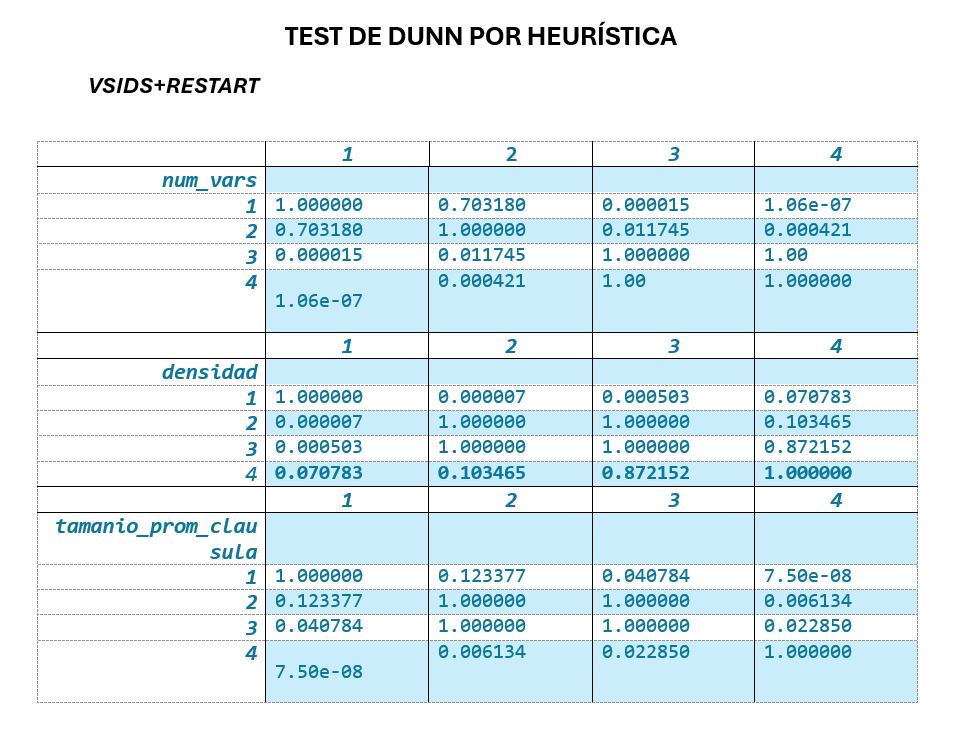
\includegraphics[width=0.8\textwidth]{Graphics/test_dunn_vsids_restart.png}
    \caption{Test Dunn por cuartiles para VSIDS con restart.}
    \label{fig:test-dunn-vsids-restart}
\end{figure}

\begin{figure}[ht]
    \centering
    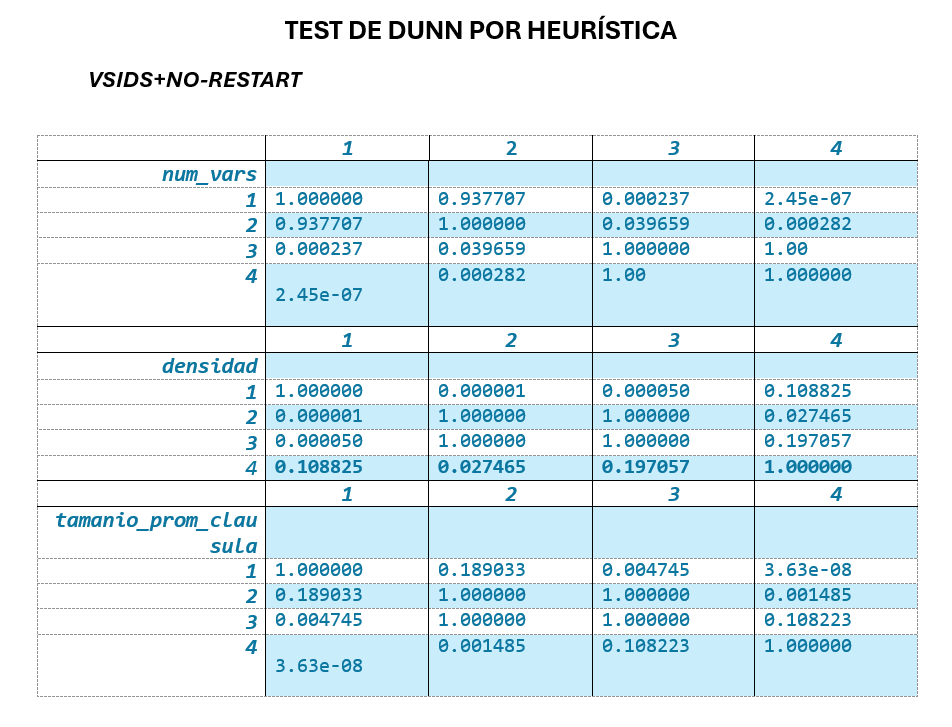
\includegraphics[width=0.8\textwidth]{Graphics/test_dunn_vsids_no_restart.png}
    \caption{Test Dunn por cuartiles para VSIDS sin restart.}
    \label{fig:test-dunn-vsids-no-restart}
\end{figure}

\begin{figure}[ht]
    \centering
    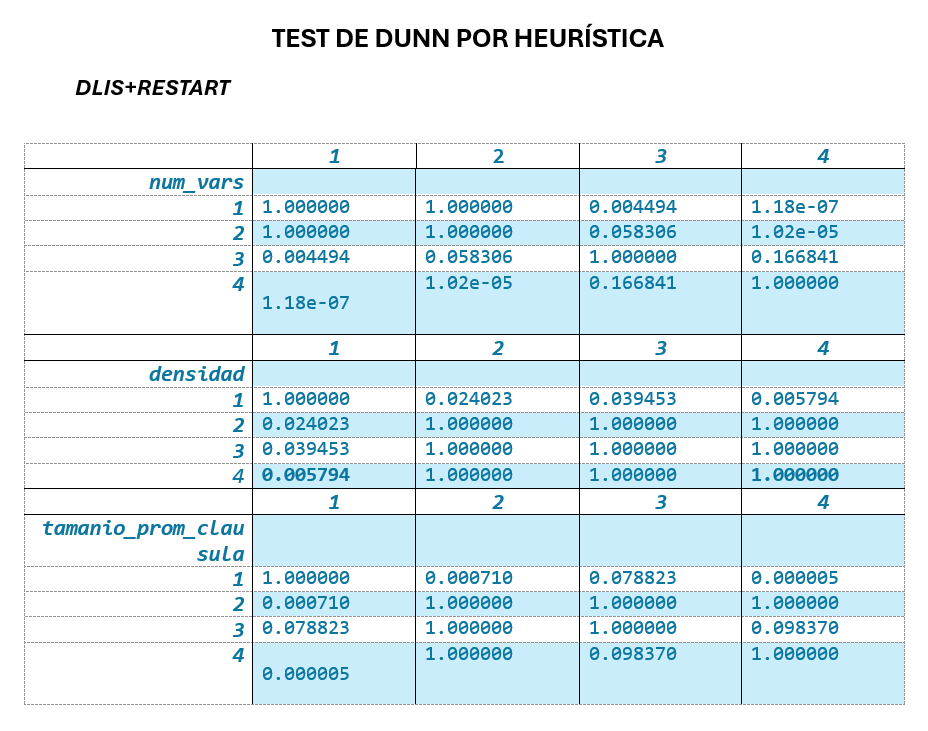
\includegraphics[width=0.8\textwidth]{Graphics/test_dunn_dlis_restart.png}
    \caption{Test Dunn por cuartiles para DLIS con restart.}
    \label{fig:test-dunn-dlis-restart}
\end{figure}

\begin{figure}[ht]
    \centering
    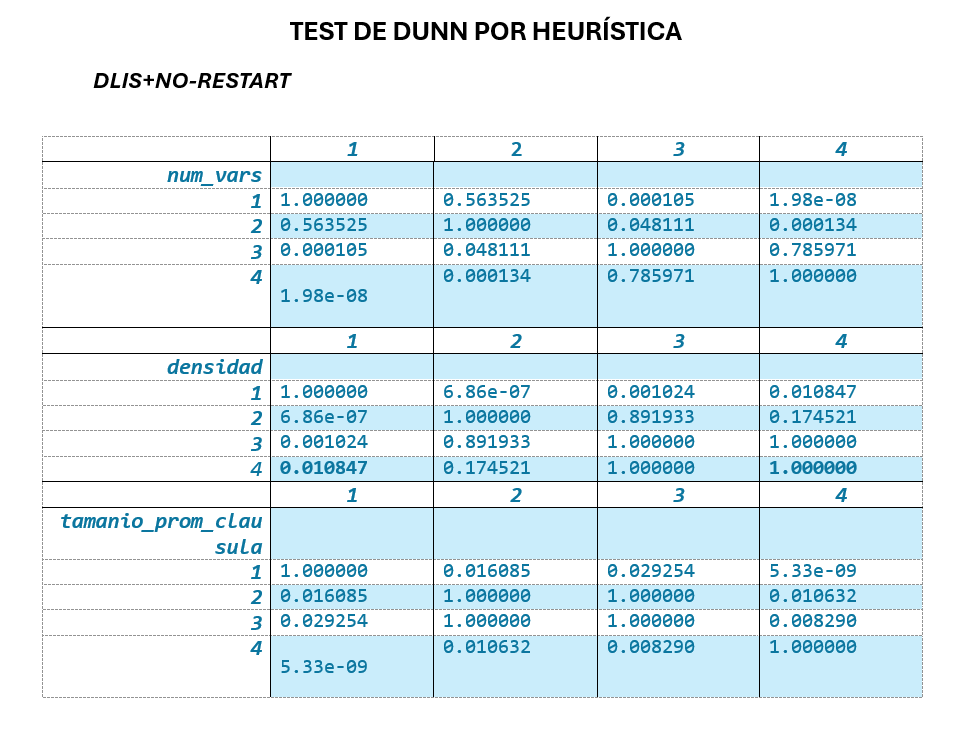
\includegraphics[width=0.8\textwidth]{Graphics/test_dunn_dlis_no_restart.png}
    \caption{Test Dunn por cuartiles para DLIS csin restart.}
    \label{fig:test-dunn-dlis-no-restart}
\end{figure}

El test post-hoc de Dunn aplicado por cuartiles (grupos definidos con ranking para evitar empates) para cada heurística y variable seleccionada permite identificar con precisión entre qué grupos existen diferencias significativas en el tiempo de resolución (logaritmo del tiempo).

En general, para la variable ``número de variables'', se observan diferencias altamente significativas entre los cuartiles extremos (por ejemplo, grupo 1 vs. 4) en todas las heurísticas, con p-valores muy bajos (p < 0.001), lo que confirma que problemas más grandes requieren tiempos significativamente mayores para resolverse. En los grupos intermedios, las diferencias son menos consistentes pero también aparecen comparaciones significativas, evidenciando una relación gradual entre tamaño y tiempo. 

Para la densidad, los resultados muestran diferencias significativas principalmente entre los cuartiles más bajos y más altos, aunque en algunos casos los grupos intermedios no difieren tanto, indicando que la densidad afecta el tiempo pero con menor fuerza y de manera menos lineal que el tamaño.

En cuanto al tamaño promedio de cláusula, también se detectan diferencias significativas entre los extremos, especialmente entre el primer y cuarto cuartil, y en varios casos entre grupos adyacentes, lo que sugiere que esta variable influye en el rendimiento, aunque su efecto puede ser más sutil o no monotónico.

La consistencia de estos patrones a lo largo de todas las heurísticas refuerza la importancia de estas características para explicar la variabilidad en el tiempo de resolución.



\backmatter

\begin{conclusions}
El dilema en CDCL
CDCL mitiga parcialmente este problema mediante el aprendizaje de cláusulas, pero no elimina la dependencia de la selección inicial de variables. Por ejemplo:

Si VSIDS elige variables periféricas en un problema con núcleos críticos (ej: PHP), el solver gastará recursos en regiones irrelevantes.

Si DLIS prioriza literales frecuentes en problemas con restricciones jerárquicas (ej: scheduling), perderá la capacidad de explotar correlaciones locales.

Esta interdependencia entre heurísticas y estructura del problema explica por qué, a pesar de los avances en CDCL, no existe una estrategia universalmente óptima. La selección de variables sigue siendo un cuello de botella teórico y práctico, especialmente al escalar a miles de variables con relaciones complejas.

La introducción de CDCL marcó un avance al reemplazar el retroceso (backtrack) cronológico con uno dirigido por conflictos, pero su éxito está ligado a la sinergia entre aprendizaje y selección de variables. Mientras las cláusulas aprendidas reducen el espacio de búsqueda, las heurísticas de selección determinan cómo se navega en él. Un desbalance entre estos componentes condena al solver a un rendimiento subóptimo, perpetuando la necesidad de estudios comparativos como el propuesto en esta tesis. 
\end{conclusions}

\begin{recomendations}
    Recomendaciones
\end{recomendations}

\printbibliography[heading=bibintoc]


\end{document}